%====================================================================================================
% Monitoramento de servidores Linux por web sites.
%====================================================================================================
% TCC
%----------------------------------------------------------------------------------------------------
% Autor				    : Eduardo Balan
% Orientador		  : Kleber Krugrer
% Instituição 		: UFMS - Universidade Federal do Mato Grosso do Sul
% Departamento		: CPCX - Sistema de Informação
%----------------------------------------------------------------------------------------------------
% Data de criação	: 29 de Março de 2017
%====================================================================================================

\documentclass[a4paper,12pt,brazil]{dct-class}

\usepackage[utf8]{inputenc}
\usepackage[top=30mm,bottom=25mm,left=25mm,right=20mm]{geometry}

\usepackage{caption}
\usepackage{subcaption}
\usepackage{pdfpages}
\usepackage[utf8]{inputenc}
\usepackage[T1]{fontenc}
\usepackage[brazil]{babel}
%\usepackage{pdfpages}

\usepackage{listings} % exibe codigos de linguagens

%Configura as linguagens de programação, java, c++ e latex

\usepackage{xcolor}
% Definindo novas cores
\definecolor{verdecpp}{rgb}{0,0.5,0}
\definecolor{verdejava}{rgb}{0.25,0.5,0.35}
\definecolor{jpurple}{rgb}{0.5,0,0.35}

%% para usar varias linguagens use \lstdefinestyle{}
\lstdefinestyle{LaTeX}{
  language={[LaTeX]TeX},
  basicstyle=\ttfamily\small, 
  identifierstyle=\color{black}, 
  keywordstyle=\color{blue}, 
  commentstyle=\color{red}, 
  extendedchars=true, 
  showspaces=false, 
  showstringspaces=false, 
  numbers=none,
  %numberstyle=\tiny,
  breaklines=true, 
  backgroundcolor=\color{yellow!20}, 
  breakautoindent=true, 
  captionpos=b,
  xleftmargin=0pt,
  frame=none,   %%frame=single
  rframe={},
	tabsize=10
}

\lstdefinestyle{CPP}
{
  language=C++,
	basicstyle=\ttfamily\small,
  alsolanguage={[Sharp]C},
  basicstyle=\ttfamily\small, 
  keywordstyle=\color{blue}, 
  stringstyle=\color{verdecpp}, 
  commentstyle=\color{red}, 
  extendedchars=true, 
  showspaces=false, 
  showstringspaces=false, 
  numbers=left,
  numberstyle=\tiny,
  breaklines=true, 
  backgroundcolor=\color{green!10},
  breakautoindent=true, 
  captionpos=b,
  xleftmargin=0pt,
	tabsize=10
}

% XML style
\definecolor{dkgreen}{rgb}{0,0.6,0}
\definecolor{gray}{rgb}{0.5,0.5,0.5}
\definecolor{mauve}{rgb}{0.58,0,0.82}
\definecolor{gray}{rgb}{0.4,0.4,0.4}
\definecolor{darkblue}{rgb}{0.0,0.0,0.6}
\definecolor{lightblue}{rgb}{0.0,0.0,0.9}
\definecolor{cyan}{rgb}{0.0,0.6,0.6}
\definecolor{darkred}{rgb}{0.6,0.0,0.0}

\lstdefinestyle{XML}
{
	basicstyle=\ttfamily\small,
	extendedchars=true, 
  showspaces=false, 
  showstringspaces=false, 
  numbers=left,
  numberstyle=\tiny,
  breaklines=true, 
  morestring=[s][\color{mauve}]{"}{"},
  morestring=[s][\color{black}]{>}{<},
  morecomment=[s]{<?}{?>},
  morecomment=[s][\color{dkgreen}]{<!--}{-->},
  stringstyle=\color{black},
  identifierstyle=\color{lightblue},
  keywordstyle=\color{red},
  morekeywords={xmlns,xsi,noNamespaceSchemaLocation,type,id,x,y,source,target,version,tool,transRef,roleRef,objective,eventually}% list your attributes here
	tabsize=10
}
		
		
\lstdefinestyle{Java}
{
  language={Java},
  basicstyle=\ttfamily\small, 
  keywordstyle=\color{jpurple}\bfseries,
  stringstyle=\color{red},
  commentstyle=\color{verdejava},
  morecomment=[s][\color{blue}]{/**}{*/},
  extendedchars=true, 
  showspaces=false, 
  showstringspaces=false, 
  numbers=left,
  numberstyle=\tiny,
  breaklines=true, 
  backgroundcolor=\color{cyan!10}, 
  breakautoindent=true, 
  captionpos=b,
  xleftmargin=0pt,
  tabsize=10
}

\lstdefinestyle{LIVRE}
{
  basicstyle=\ttfamily\small, 
  extendedchars=true, 
  showspaces=false, 
  showstringspaces=false, 
  numbers=left,
  numberstyle=\tiny,
  breaklines=true, 
  breakautoindent=true, 
  captionpos=b,
  xleftmargin=0pt,
  tabsize=10
}



\usepackage{setspace}
%\usepackage{caption}
\usepackage[font=small]{caption}

%\DeclareCaptionFormat{myformat}{#1#2#3\hrulefill}
%\captionsetup{format=myformat}
%\captionsetup[lstlisting]{position=bottom}
%\captionsetup[lstinputlisting]{position=bottom,format=myformat}

\usepackage{multicol}

\usepackage{booktabs}	% http://ctan.org/pkg/booktabs
\usepackage{array}		% http://ctan.org/pkg/array
\newcolumntype{M}{>{\centering\arraybackslash}m{\dimexpr.25\linewidth-2\tabcolsep}}

\begin{document}

\thispagestyle{empty}
%====================================================================================================
% Monitoramento de servidores Linux por web sites.
%====================================================================================================
% TCC
%----------------------------------------------------------------------------------------------------
% Autor				    : Eduardo Balan
% Orientador		  : Kleber Krugrer
% Instituição 		: UFMS - Universidade Federal do Mato Grosso do Sul
% Departamento		: CPCX - Sistema de Informação
%----------------------------------------------------------------------------------------------------
% Data de criação	: 29 de Março de 2017
%====================================================================================================

\titulo{Trabalho de Conclusão de Curso\vskip 1.0cm
API para monitoramento de servidores Linux.}\vskip 0.5cm
\autor{Eduardo Balan}


\orientacao{Prof. Me. Kleber Kruger}
\textofree{\large Bacharelado em Sistemas de Informação}


\vfill \centerline{
\includegraphics[scale=0.15]{figuras/ufms-logo.jpg}}

\vskip 0.5cm
\begin{center}
Sistema de Informação\\
Universidade Federal de Mato Grosso do Sul\\
15 de dezembro de 2017
\end{center}
		

\chapter*{}

\begin{center}

\begin{minipage}[t]{10cm}
	\begin{center}
		\vspace{-2cm}
		%{{\Large Monitoramento de servidores Linux utilizando arquitetura cliente-servidor.}} 
		{{\Large API para monitoramento de servidores Linux.}} 
	\end{center}
\end{minipage}

\end{center}


\begin{flushright}
	\vspace{12cm}
	Coxim, 15 de dezembro de 2017.
	
\end{flushright}

\vspace{2cm}
Banca Examinadora:

\begin{itemize}
	\item Prof. Me. Kleber Kruger (CPCX/UFMS) - Orientador
	\item Prof. %Dr. Gedson Faria (CPCX/UFMS)
	\item Prof. %Esp. Gustavo Yoshio Maruyama (CPCX/IFMS)
\end{itemize}

%====================================================================================================
% Monitoramento de servidores Linux por web sites.
%====================================================================================================
% Plano de Trabalho
%----------------------------------------------------------------------------------------------------
% Autor					: Eduardo Balan
% Orientador		: Kleber Kruger
% Instituição 	: UFMS - Universidade Federal do Mato Grosso do Sul
% Unidade				: CPCX - Campus de Coxim
%----------------------------------------------------------------------------------------------------
% Arquivo			: plano_trabalho.tex
% Data de criação	: 29 de Março de 2017
%=====================================================================================================

\chapter*{Resumo}

 % Resumo
%====================================================================================================
% Monitoramento de servidores Linux por web sites.
%====================================================================================================
% Plano de Trabalho
%----------------------------------------------------------------------------------------------------
% Autor					: Eduardo Balan
% Orientador		: Kleber Kruger
% Instituição 	: UFMS - Universidade Federal do Mato Grosso do Sul
% Unidade				: CPCX - Campus de Coxim
%----------------------------------------------------------------------------------------------------
% Arquivo			: plano_trabalho.tex
% Data de criação	: 29 de Março de 2017
%=====================================================================================================

\chapter*{Abstract}

The web has been increasingly used as a way to run applications. There are currently word processors, spreadsheets and other programs running as a web application, where your main information is stored on the servers \cite{Marimoto:2011}. It's easy to realize that a server crash can compromise user productivity, mainly if that server is the only one available or running vital services \cite{Weber:2002}.

The main objective of this work was to study about technologies such as Linux, C ++, Java, Spring and PostgreSQL to create a monitoring system for Linux servers using the client-server architecture. Another goal was to automatically perform backup and vacuum procedures on the PostgreSQL database. These procedures are of great importance to identify problems, once these servers can store vital data such as financial data, user accounts, corporate reports, software and hardware projects, among others.

In the implementation part, it was developed a system called MonitorWeb, consisting of two applications: the first, a client application called MonitorWeb-Cli, which performs monitoring of CPU, memory and swap at intervals defined according to the user, besides allow backup and vacuum procedures to be performed in sporadic times. The second consists of a web service that receives the monitoring data from the client applications and provides the informations through the ReST standard so that other applications can use them.

Finally, the results are described, to which the client application was submitted 15 times (10 times for 1-second interval monitoring and 5 for no intervals) to the Valgrind tool, in order to identify problems of memory leakage and inefficient allocation of resources. In the end, no problem was detected. The server application was subjected to a load of 86 unit tests, ensuring that all the resources work with greater reliability. Two test batteries were also runned: the first with common settings to a real environment (interval monitoring of 1-second) to check the performance. The second defined a configuration without interval between the monitoring, and was performed in order to check the performance of the server when exposed to an excessive load of requests per second. Both tests presented satisfactory results, having the second an average insertion rate of 546.34 records per second. % Abstract
%%====================================================================================================
% Monitoramento de servidores Linux por web sites.
%====================================================================================================
% Plano de Trabalho
%----------------------------------------------------------------------------------------------------
% Autor					: Eduardo Balan
% Orientador		: Kleber Kruger
% Instituição 	: UFMS - Universidade Federal do Mato Grosso do Sul
% Unidade				: CPCX - Campus de Coxim
%----------------------------------------------------------------------------------------------------
% Arquivo			: plano_trabalho.tex
% Data de criação	: 29 de Março de 2017
%=====================================================================================================

\chapter{Agradecimentos} \label{Cap:Agradecimentos}


Agradeço 

Agradeço ao meu amigo Bel. Cleiton Gonçalves de Almeida por solucionar algumas duvidas sobre o Spring Boot.

Agradeço ao meu amigo Rafael por me ajudar a realizar os testes apresentados neste trabalho.

Agradeço principalmente ao meu orientador Me. Kleber Kruger pois sem a sua dedicação eu não teria conseguido. % Abstract


\tableofcontents

%\printglossaries

\cleardoublepage
\phantomsection
\addcontentsline{toc}{chapter}{Lista de Figuras}
\listoffigures

\cleardoublepage
\phantomsection
\addcontentsline{toc}{chapter}{Lista de Tabelas}
\listoftables

%\cleardoublepage
%\phantomsection
%\addcontentsline{toc}{chapter}{Lista de Algoritmos}
%\listofalgorithmes

\cleardoublepage
\phantomsection
\addcontentsline{toc}{chapter}{Lista de Quadros}
\lstlistoflistings

% lista de abreviaturas e siglas
% o parametro deve ser a abreviatura mais longa
%\begin{listofabbrv}{SPMD}
%	\item[CMM] Capability Maturity Model
%	\item[SMP] Symmetric Multi-Processor
%	\item[NUMA] Non-Uniform Memory Access
%	\item[SIMD] Single Instruction Multiple Data
%	\item[SPMD] Single Program Multiple Data
%	\item[ABNT] Associação Brasileira de Normas Técnicas
%\end{listofabbrv}

%\pdfbookmark[0]{\lstlistlistingname}{lol}
%\begin{KeepFromToc}
%\lstlistoflistings
%\end{KeepFromToc}
%\cleardoublepage

% Monitoramento de servidores Linux por web sites.
%====================================================================================================
% TCC
%----------------------------------------------------------------------------------------------------
% Autor				    : Eduardo Balan
% Orientador		  : Kleber Krugrer
% Instituição 		: UFMS - Universidade Federal do Mato Grosso do Sul
% Departamento		: CPCX - Sistema de Informação
%----------------------------------------------------------------------------------------------------
% Data de criação	: 29 de Março de 2017
%====================================================================================================

\chapter{Introdução} \label{Cap:Introducao}

A Internet é uma rede de computadores que interconecta milhares de dispositivos computacionais ao redor do mundo com centenas de milhares de usuários. Há pouco tempo, esses dispositivos eram basicamente computadores de mesa e servidores que realizavam diversas tarefas, como armazenamento e distribuição de dados e arquivos, gerenciamento de impressão e de usuários, conexão a outras redes, transmissão de informações tais como páginas da \textit{web} e mensagens de e-mail, além de outras funcionalidades \cite{Kurose:2010}. Com frequência, essas máquinas assim chamadas servidores são instaladas e mantidas em um local central de uma empresa por um administrador de sistemas \cite{Tanenbaum:2003}. 

Nos últimos tempos houve uma mudança, que é o uso da \textit{web} não apenas para comunicação, mas como uma forma de executar aplicativos.  Agora temos processadores de texto, planilhas e outros programas sendo executados como uma aplicação \textit{web} em um navegador, em que suas principais informações ficam armazenadas nos servidores \cite{Marimoto:2011}. Uma vez que os dados dos usuários estão armazenados em locais remotos algumas vantagens podem ser obtidas, tais como \textit{self-service} sob demanda e amplo acesso à rede, \cite{Sampaio:2003}  mas por outro lado, manter estes dados seguros é imprescindível e o acompanhamento destes servidores é uma forma de garantia. É fácil perceber que a queda de um servidor pode comprometer a produtividade de usuários, principalmente se esse servidor for o único disponível ou se estiver executando serviços vitais \cite{Weber:2002}.

Cabe observar, que segundo Carlos E. Marimoto, pouco a pouco, a internet tem se tornado o verdadeiro computador, e os computadores passam a ser cada vez mais um simples terminal, cuja única função é mostrar informações processadas por servidores remotos. Isso se tornou possível devido à popularização da ADSL (\textit{Assymetrical Digital Subscriber Line}), \textit{wireless} e outras formas de acesso rápido e contínuo à internet. Futuramente, a tendência é que mais aplicativos passem a ser usados via \textit{web}, tornando um computador desconectado cada vez mais limitado e inútil. Eventualmente, é possível que o próprio computador seja substituído por dispositivos mais simples e baratos, que sirvam como terminais de acesso \cite{Marimoto:2011}.

\section{Justificativa}

Muitas empresas detêm valiosas informações guardadas em seus servidores, que podem ser de ordem técnica (por exemplo, o projeto de um novo \textit{chip} ou novo \textit{software}), comercial (como estudos sobre competidores ou planos de \textit{marketing}), financeira (planos para uma venda de ações), jurídica (documentos sobre uma possível fusão ou aquisição), entre outras possibilidades. Além das ameaças causadas por invasores, dados valiosos podem ser perdidos por acidente. Algumas das causas comuns de perda acidental de dados são fenômenos naturais, como enchentes, terremotos, guerras, motins; erros de hardware ou de software (defeitos na CPU, discos ou fitas com problemas de leitura, surtos ou falhas de energia, sujeira,  erros de programas e temperaturas extremas); e erros humanos (entrada incorreta de dados, montagem incorreta de disco ou fita, execução de programas errado, entre outro) \cite{Tanenbaum:2010,Silberschatz:2000}.


Em 27 de dezembro de 2005, um incêndio destruiu seis dos dez andares do  prédio do INSS (Instituto Nacional de Seguro Social), em  Brasília \cite{Laudo:2006}. Segundo o ministro da Previdência e Assistência Social da época, Nelson Machado, as maiores perdas foram de informações de receita previdenciária, informações do sistema central e processos físicos, dívidas de empresas, processos de fraudes e autos de infração \cite{Machado:2005}. O presidente da Comissão de Fiscalização e Controle da Câmara dos Deputados, deputado Alexandre Cardoso, estimou, que os prejuízos, naquela época, referentes à processos administrativos foram equivalentes a R\$ 60 bilhões, tendo a previdência cópias de pelo menos R\$ 53 bilhões, concluindo que a união teria perdido em torno de R\$7 bilhões \cite{Futema:2005}.


A maioria dessas causas podem ser tratadas com a manutenção adequada dos \textit{backups}, preferivelmente em lugar distante dos dados originais. Embora proteger dados de perda acidental possa parecer banal, se comparado a proteger contra invasores inteligentes, na prática provavelmente mais danos são causados pelo primeiro que pelo ultimo \cite{Tanenbaum:2003, Silberschatz:2000}.

\section{Objetivos} \label{Sec:Objetivos}

\subsection{Objetivo Geral} \label{Sec:ObjetivoGeral}

O objetivo deste trabalho é estudar as formas utilizadas para prevenir erros, e aplicar esse técnicas na  criação de ferramentas de monitoramento para servidores. Todas as informações de monitoramento ficarão a disposição de seus usuários através de um \textit{web} site central, facilitando o trabalho de acompanhamento das rotinas dos servidores, e prevenções de problemas futuros.


\subsection{Objetivos Específicos}\label{Sec:ObjetivosEspecificos}
\begin{itemize}
	\item Pesquisar as principais formas utilizadas para prevenir os erros em servidores e identificando os pontos mais vulneráveis.
	
	\item Estudar como fazer leituras de informações do hardware,  tais como dados dos discos rígidos, processador, memória, temperatura da placa mãe, etc...
	
	\item	Criar um \textit{web} site para visualizar as informações dos servidores.

	\item Criar uma API para sincronizar as informações entre o sistema e \textit{web} site.
\end{itemize}


\newpage

\section{Organização da Proposta} \label{Sec:Organizacao}

xxxxxxxxxxxxxxxxxxxxxxxxxxxxxxxxxxxxxxxxxxxxxxxxxxxxxxxxxxxxxxxxxxxxxxxxxxxxxxxxxxxx
No Capítulo 2 são apresentados os conceitos utilizados neste trabalho de acordo com a literatura estudada. Na Seção \ref{sec:falhaErroDefeito} explica-se os conceitos de falha, erro e defeito ou modelo de três universos. Na Seção \ref{sec:radiacao} são descritas as principais fontes de radiação e seus efeitos nos circuitos eletrônicos.  O conceito de ``dependabilidade'' é explicado na Seção \ref{sec:denpendabilidade} e na Seção \ref{sec:tolerancia} explica-se o conceito geral de tolerância a falhas e os atributos necessários para que uma falha seja definida. Na seção \ref{sec:tecnica} são apresentadas as principais técnicas de tolerância a falhas e na seção \ref{sec:InjecaoDeFalhas} as principais técnicas de injeção de falhas.

As modificações realizadas nas bibliotecas e a criação da classe \textit{TData} são exibidas no Capítulo 3, dividido em três seções. Na Seção \ref{sec:InjetorDeFalhas} são apresentadas as implementações e as modificações realizadas na biblioteca \textit{FaultInjector}. Na Seção \ref{sec:extensaoBiblioteca} é exibida a extensão da biblioteca \textit{FaultRecovery}. Na Seção \ref{sec:classeTData} são exibidas as implementações realizadas para criação da classe \textit{TData}, sua utilização é explicada mediante exemplos.

No Capítulo \ref{cap:Resultados} são exibidos os resultados encontrados após os testes de tempo de execução e tolerância a falhas em que foram expostas as bibliotecas \textit{FaultInjector}, \textit{FaultRecovery} e a classe \textit{TData}. No Capítulo \ref{cap:conclusao} são exibidas as considerações finais deste trabalho.
xxxxxxxxxxxxxxxxxxxxxxxxxxxxxxxxxxxxxxxxxxxxxxxxxxxxxxxxxxxxxxxxxxxxxxxxxxxxxxxxxxxxxx

 % Introdução
% Monitoramento de servidores Linux por web sites.
%====================================================================================================
% TCC
%----------------------------------------------------------------------------------------------------
% Autor				    : Eduardo Balan
% Orientador		  : Kleber Krugrer
% Instituição 		: UFMS - Universidade Federal do Mato Grosso do Sul
% Departamento		: CPCX - Sistema de Informação
%----------------------------------------------------------------------------------------------------
% Data de criação	: 29 de Março de 2017
%====================================================================================================

\chapter{Fundamentação Teórica}\label{cap:funTeorica}

Neste Capítulo são apresentados os conceitos utilizados neste trabalho de acordo com a literatura estudada. Na seção \ref{sec:ArquiteturaClienteServidor} explica-se os conceitos da arquitetura cliente-servidor. Na Seção \ref{sec:WebServices} explicase os conceitos de um \textit{web-service}. Na Seção \ref{sec:BancodeDados} explica-se o conceito de Banco de Dados. Na Seção \ref{sec:Http} explica-se o conceito do protocolo HTTP/1.1 seus metodos forma de utilização e respostas esperadas. Na Seção \ref{sec:ArquiteturaReST} é apresentada o estilo de desenvolvimento da arquitetura ReST e na Seção \ref{sec:TestesAutomatizados} são mostradas as principais vantagens e melhorias adquiridas por meio dos testes automatizados.


\section{Arquitetura Cliente-Servidor}\label{sec:ArquiteturaClienteServidor}

		Em uma arquitetura cliente-servidor há um hospedeiro sempre em funcionamento, denominado servidor, que atende à requisições de muitos outros hospedeiros, denominados clientes. Estes podem estar em funcionamento esporadicamente ou a todo o tempo. Um exemplo clássico é a aplicação \textit{web} na qual um servidor \textit{web} que está sempre em funcionamento atende à requisições de \textit{browsers} de hospedeiros clientes. Ao receber uma requisição de um objeto de um hospedeiro cliente, o servidor \textit{web} responde enviando o objeto requisitado a ele. Observe que, na arquitetura cliente-servidor, os clientes não se comunicam diretamente uns com os outros: por exemplo, na aplicação \textit{web}, dois \textit{browsers} não se comunicam diretamente. Outra característica da arquitetura cliente-servidor é que o servidor tem um endereço fixo, bem conhecido, denominado endereço IP (\textit{Internet Protocol}). Devido a esse característica do servidor e devido ao fato de ele estar sempre em funcionamento, um cliente sempre pode contatá-lo enviando um pacote ao endereço do servidor. Algumas das aplicações mais conhecidas que empregam a arquitetura cliente-servidor são \textit{web}, FTP (\textit{File Transfer Protocol}), Telnet e e-mail. Essa arquitetura cliente-servidor é mostrada na \autoref{Img:ArquiteturaClienteServidor} em que diversos clientes utilizando, computadores, notebooks e celulares realizam comunicação com um servidor \cite{Kurose:2010}.

Em aplicações cliente-servidor, muitas vezes acontece de um único hospedeiro servidor ser incapaz de atender a todas as requisições de seus clientes. Um site \textit{web} pode ficar rapidamente saturado se tiver apenas um servidor para atender grande número de requisições. Por essa razão, um grande conjunto de hospedeiros - às vezes coletivamente chamados \textit{data center} - freqüentemente é usado para criar um servidor virtual poderoso em arquitetura cliente-servidor, aumentando a capacidade de resposta de requisições \cite{Kurose:2010}.


\begin{figure}
	\centering
	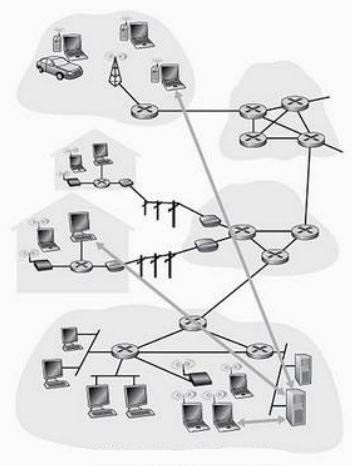
\includegraphics[width=0.5\textwidth]{figuras/KuroseClienteServidorpg88.jpg}
	\caption[Arquitetura Cliente-Servidor.]{Representa a arquitetura clitente-Servidor, onde diversos tipos de cliente se comunicam com um mesmo servidor.}
	\label{Img:ArquiteturaClienteServidor}
\end{figure}


\section{\textit{Web Services}}\label{sec:WebServices}


O \textit{Web Service} é um \textit{software}  que atende a uma função de negócio específica para seus clientes. Ele recebe requisições de clientes e as responde ocultando todo o detalhamento do seu processamento. Normalmente as transações estão em formato XML (\textit{Extended Markup Language}), e são transmitidas utilizando o protocolo HTTP (HyperText Transfer Protocol), entretanto podem ser utilizados outros protocolos de transporte \cite{Sampaio:2003}.

Os \textit{Web Services}, aliados aos padrões estabelecidos da Internet, podem fazer com que os dados fluam entre as várias entidades, como o governo e empresas interagindo entre si, reduzindo custos de modo a possibilitar maior facilidade e rapidez na troca de informações \cite{Abinader:2006}. Um exemplo utilizado nacionalmente é a NF-e (Nota Fiscal Eletrônica) em que diversas empresas com \textit{softwares} diferentes enviam arquivos xml utilizando o protocolo https (\textit{Hyper Text Transfer Protocol Secure}) para o \textit{web service} da receita federal, aguardam a realização dos processamentos de validação e recebem um arquivo xml de retorno com as informações desejadas.

Um \textit{web wervice} deve executar unidades completas de trabalho, não dependendo do estado de outros componentes externos. Outra definição importante é que eles devem ser "\textit{Stateless}" ou seja, cada requisição é considerada uma transação independente que não está relacionada a qualquer requisição anterior de forma que a comunicação consista de pares de requisição e resposta independentes \cite{Sampaio:2003, W3C:2001}.


\section{Banco de Dados} \label{sec:BancodeDados}

Um Sistema de banco de dados é basicamente um sistema computadorizado de manutenção de registros. O banco de dados, por si só, pode ser considerado como o equivalente eletrônico de um armário de arquivamento; ou seja, ele é um repositório ou recipiente para uma coleção de arquivos de dados computadorizados. Os usuários de um banco de dados podem solicitar que o sistema realize diversas operações envolvendo tais arquivos, por exemplo:
\begin{itemize}
		\item Acrescentar novos arquivos ao banco de dados
		\item Inserir dados em arquivos existentes 
		\item Buscar dados de arquivos existentes
		\item Excluir dados de arquivos existentes
		\item Alterar dados em arquivos existentes
		\item Remover arquivos existentes do Banco de dados
\end{itemize}

As informações contidas no banco de dados em questão podem ser qualquer coisa que tenha algum significado ou indivíduo ou à organização a que o sistema deve servir, ou seja, qualquer coisa que seja necessária para auxiliar no processo geral das atividades desse indivíduo ou dessa organização

Os sistemas de bancos de dados Estão disponíveis em máquinas que variam desde pequenos computadores de mão (hand-helds e celulares) ou computadores pessoais até os maiores mainframes ou clusters de computadores de grande porte. Normalmente sistemas em máquinas grandes costumam ser multiusuários, enquanto os que estão em máquinas menores tendem a ser de monousuários. Um sistema monousuário é um sistema em que no máximo um usuário pode acessar o banco de dados em determinado momento; um sistema multiusuário é aquele em que muitos usuários podem acessar o banco de dados ao mesmo tempo; porém, a distinção é irrelevante para a maioria dos usuários, pois um dos objetivos dos sistemas multiusuários, em geral, é que cada usuário se comporte como se estivesse trabalhando com um sistema monousuário.


As informações contidas no banco de dados são persistentes, ou seja, uma vez que um operação de inserir é aceita pelo SGBD (Sistema de Gerenciamento de Banco de Dados), ela só poderá ser removida por outra requisição explicita ao SGBD, e não como um mero efeito colateral, como algum programa concluindo sua execução apagar todos os registros.


As transações realizadas pelo SGBD utilizam o conceito de ACID(Atomicidade, Consistência, Isolamento e Durabilidade):

\begin{itemize}
		\item Atomicidade quer dizer que um bloco de transações deve ter todas as suas operações executadas em caso de sucesso ou nenhum operação executada, mesmo que o sistema venha a falha.
		\item Consistência diz que a execução de uma transação deve levar o banco de dados de um estado consistente a um outro estado consistente, dessa forma, uma transação deve respeitar as regras de integridade dos dados
		\item Isolamento quer dizer que transações paralelas não interferem umas nas outras, ou seja, se um usuário tentar alterar o salario de um funcionário e outro usuário tentar alterar o mesmo salario ao mesmo tempo uma transação só iniciara quando a outra for completamente terminada.
		\item Durabilidade diz que as transações com sucesso devem persistir no banco de dados mesmo em caso de falha.
\end{itemize}



\section{HTTP/1.1 \textit{HyperText Transfer Protocol}} \label{sec:Http}

O protocolo HTTP (\textit{HyperText Transfer Protocol}) é o protocolo utilizado em toda a \textit{World Wide Web}. Ele especifica o formato das mensagens que os clientes enviam aos servidores e também o formato de respostas que receberão. Cada interação consiste em uma solicitação ASCII, seguida por uma resposta RFC 822. 

Na utilização do protocolo HTTP/1.1 todos os clientes e todos os servidores devem obedecer a esse protocolo que é definido na RFC 2616 \cite{Tanenbaum:2003}.

\subsection{Conexões} \label{HTTP/1.1 - HyperText Transfer Protocol}

O modo habitual de cliente entrar em contato com um servidor é estabelecer uma conexão TCP (\textit{Transmission Control Protocol}) para a porta 80 da máquina servidora, embora esse procedimento não seja exigido formalmente. A vantagem de se usar o TCP é que ambas as partes não têm de se preocupar com mensagens perdidas, mensagens duplicadas, mensagens longas ou confirmações. Todos esses assuntos são tratados pela implementação do TCP \cite{Tanenbaum:2003}.

O HTTP/1.1 diferentemente de seus antecessores, admite conexões persistentes. Com elas, é possível estabelecer uma conexão TCP, enviar uma solicitação e obter uma resposta, e depois enviar solicitações adicionais e receber respostas adicionais. Amortizando o custo da instalação e
da liberação do TCP por várias solicitações, o processamento relativo devido ao TCP é muito menor por solicitação. Também é possível transportar as solicitações por \textit{pipeline}, ou seja, enviar a segunda solicitação antes de chegar a resposta da primeira \cite{Tanenbaum:2003}.



\subsection{Métodos} \label{subsec:Metodos}

O HTTP foi criado de modo mais geral que simplesmente para utilização na \textit{web}, visando às futuras aplicações orientadas a objetos. Por essa razão, são aceitas operações chamadas métodos, diferentes da simples solicitação de uma página da \textit{web}. Cada solicitação consiste em uma ou mais linhas de texto ASCII, sendo a primeira palavra da primeira linha o nome do método solicitado. Os métodos internos estão listados na \autoref{Tab:MetodosHTTP} \cite{Tanenbaum:2003}.


% Please add the following required packages to your document preamble:
% \usepackage[table,xcdraw]{xcolor}
% If you use beamer only pass "xcolor=table" option, i.e. \documentclass[xcolor=table]{beamer}
\begin{table}[!ht]
\centering
\begin{tabular}{|l|l|}
\hline
{\color[HTML]{000000} \textbf{Método}} & {\color[HTML]{000000} \textbf{Descrição}} 
\\ \hline
GET                                    & \multicolumn{1}{p{13.50cm}|}{O método GET solicita ao servidor que envie a página (ou objeto, no caso mais genérico; na prática,apenas um arquivo). A grande maioria das solicitações a servidores da \textit{web} tem a forma de métodos GET.} 
\\ \hline
HEAD                                   & \multicolumn{1}{p{13.50cm}|}{O método HEAD solicita apenas o cabeçalho da mensagem, sem a página propriamente dita. Essemétodo pode ser usado para se obter a data da última modificação feita na ágina, para reunirinformações destinadas à indexação, ou apenas para testar a validade de um URL(Uniform Resource Locator).}
\\ \hline
PUT                                    & \multicolumn{1}{p{13.50cm}|}{O método PUT grava em uma página já existe. Esse método possibilita a criação de um conjunto de páginas da \textit{web} em um servidor remoto. O corpo da solicitação contém a página. } 
\\ \hline
POST                                   & \multicolumn{1}{p{13.50cm}|}{O método POST grava novos dados e são "anexados" a ele, em um sentido mais genérico\cite{Tanenbaum:2003}.} 
\\ \hline
DELETE                                 & \multicolumn{1}{p{13.50cm}|}{O método DELETE exclui a página. Não há garantia de que DELETE tenha sido bem-sucedido pois, mesmo que oservidor HTTP remoto esteja pronto para excluir a página, o arquivo subjacente pode ter um modoque impeça o servidor HTTP de modificá-lo ou excluí-lo \cite{Tanenbaum:2003}. }
\\ \hline
TRACE                                  & \multicolumn{1}{p{13.50cm}|}{O método TRACE serve para depuração. ele instrui o servidor a enviar de volta a solicitação. Essemétodo é útil quando as solicitações não estão sendo processadas corretamente e o cliente desejasaber qual solicitação o servidor recebeu de fato \cite{Tanenbaum:2003}.}   
\\ \hline
CONNECT                                & \multicolumn{1}{p{13.50cm}|}{O método CONNECT não é usado atualmente. Ele é reservado para uso futuro \cite{Tanenbaum:2003}.} \\ \hline
OPTIONS                                & \multicolumn{1}{p{13.50cm}|}{O método OPTIONS fornece um meio para que o cliente consulte o servidor sobre suas propriedades ou sobre as de um arquivo específico \cite{Tanenbaum:2003}.}
\\ \hline
\end{tabular}
\caption[Métodos da solicitações HTTP.]{Métodos da solicitações HTTP e suas descrições \cite{Tanenbaum:2003}.}
\label{Tab:MetodosHTTP}
\end{table}





\subsection{Códigos de Resposta} \label{subsec:Resposta}

Toda solicitação obtém uma resposta que consiste em uma linha de status e, possivelmente,
informações adicionais (por exemplo, uma página da \textit{web} ou parte dela). A linha de status contém
um código de status de três dígitos informando se a solicitação foi atendida e, se não foi, o motivo. 
O primeiro dígito é usado para dividir as respostas em cinco grupos importantes, como mostra-se na \autoref{Tab:FalhasHTTP} \cite{Tanenbaum:2003}.


% Please add the following required packages to your document preamble:
% \usepackage[table,xcdraw]{xcolor}
% If you use beamer only pass "xcolor=table" option, i.e. \documentclass[xcolor=table]{beamer}
\begin{table}[!h]
\centering
%\caption{My caption}
\begin{tabular}{|l|l|}
\hline
%\multicolumn{1}{|c|}{{\color[HTML]{000000} \textbf{Código}}} & \multicolumn{1}{c|}{{\color[HTML]{000000} \textbf{Descrição}}}    \\ \hline
\textbf{Código}   & \textbf{Descrição}       																						 \\ \hline
1xx   & Raramente são usados na prática \cite{Tanenbaum:2003}.        																						 \\ \hline
2xx   & Solicitação foi tratada com sucesso \cite{Tanenbaum:2003}.            																		 \\ \hline
3xx   & \begin{tabular}[c]{@{}l@{}}Informam ao cliente que ele deve procurar em outro lugar, 
				\\ usando uma URL diferente \cite{Tanenbaum:2003}.\end{tabular} 																						\\ \hline
4xx   & \begin{tabular}[c]{@{}l@{}}Solicitação falhou devido a um erro do cliente,
				\\ como uma solicitação inválida ou uma página inexistente \cite{Tanenbaum:2003}.\end{tabular}             \\ \hline
5xx   & \begin{tabular}[c]{@{}l@{}}O próprio servidor tem um problema, seja causado por um  
				\\ erro em seu código ou por uma sobrecarga temporária \cite{Tanenbaum:2003}.\end{tabular}                  \\ \hline
\end{tabular}
\caption[Códigos de resposta da solicitação HTTP.]{Códigos de resposta da solicitação HTTP \cite{Tanenbaum:2003}.}
\label{Tab:FalhasHTTP}
\end{table}


\subsection{Exemplo de utilização do HTTP/1.1} \label{subsec:ExemploHttp}

Este protocolo foi desenvolvido de maneira a ser o mais flexível possível para comportar diversas necessidades diferentes.
Sempre que uma requisição é enviada ela segue o formato da requisições que pode ser visto no \autoref{Func:GETModelo} \cite{Saudate:2014}.

\begin{lstlisting}[label=Func:GETModelo,caption={[Formato de uma requisição HTTP]Formato de uma requisição HTTP}]
<método> <URL> HTTP/<versão>
<Cabeçalhos - Vários cabeçalhos podem ser enviados mas um em cada linha>

<corpo da requisição> 
\end{lstlisting}


Quando um GET para http://www.site.com.br/clientes é realizado uma requisição é criada como pode ser visto no \autoref{Func:GETExemplo}. Nesta requisição pode ser visto em sua primeira linha o método GET da solicitação seguido pela URL a qual esta sendo feito a solicitação e pela versão do protocolo HTTP. O servidor responsável por receber a solicitação e a porta são passado no cabeçalho da requisição precedido por "Host:". Na terceira linha pode ser visto um cabeçalho \textit{Accept}, que serve para informar ao servidor qual tipo de dados a requisição espera receber \cite{Saudate:2014}.


\begin{lstlisting}[label=Func:GETExemplo,caption={[Exemplo de uma requisição HTTP utilizando o método GET.]Exemplo de uma solicitação HTTP utilizando o método GET, para http://www.site.com.br/clientes com o pedido de uma arquivo XML de resposta.}]
GET /clientes HTTP/1.1
Host: www.site.com.br:80
Accept: text/xml
\end{lstlisting}

Assim que o servidor receber a solicitação ele ira processar as informações, e retornara uma resposta com um dos código mostrado no \autoref{Tab:FalhasHTTP}. A resposta retornada possuirá o formato mostrado no \autoref{Func:RespostaModelo} \cite{Saudate:2014}.


\begin{lstlisting}[label=Func:RespostaModelo,caption={[Formato de uma resposta HTTP]Formato de uma resposta HTTP}]
HTTP/<versão> <código de status> <descrição do código>
<cabeçalhos>
<resposta>
\end{lstlisting}


Para a solicitação mostrada no \autoref{Func:GETExemplo} uma resposta velida seria a representada pelo \autoref{Func:RespostaExemplo}.
Nesta resposta pode ser visto em sua primeira linha a versão do protocolo HTTP. seguido pelo código de resposta e descrição do código.
Na segunda linha temos um cabeçalho Content-Type que indica qual o formato da resposta, através de um tipo conhecido como \textit{Media Type}.
A terceira linha tem um cabeçalho Content-Length que informa qual o tamanho da resposta.
A partir da quarta linha temos a resposta em XML da solicitação \cite{Saudate:2014}.



\begin{lstlisting}[label=Func:RespostaExemplo,caption={[Exemplo de uma resposta HTTP com status 200.]Exemplo de uma resposta HTTP com status 200, possuindo um Content-Type:text/xml informando que a resposta é em formato XML, e a resposta a solicitação.}]
HTTP/1.1 200 OK
Content-Type: text/xml
Content-Length: 232
<clientes>
	<cliente>
		<id>1</id>
		<nome>Alexandre</nome>
		<dataNascimento>2012-12-01</dataNascimento>
	</cliente>
	<cliente>
		<id>2</id>
		<nome>Paulo</nome>
		<dataNascimento>2012-11-01</dataNascimento>
	</cliente>
</clientes>
\end{lstlisting}


\section{Arquitetura ReST} \label{sec:ArquiteturaReST}

Os princípios básicos de ReST (\textit{Representational State Transfer}) são estilos de desenvolvimento
de \textit{web services} que teve origem na tese de doutorado de Roy Fielding. 
Este, por sua vez, é co-autor de um dos protocolos mais utilizados no mundo, o HTTP/1.1 (\textit{HyperText Transfer Protocol}) \cite{Boagrio:2017} \cite{Saudate:2014}.  
Assim, é notável que o protocolo ReST é guiado pelo que seriam as boas práticas de uso do HTTP/1.1 \cite{Saudate:2014}:


Em ReST, cada recurso deve ter uma URL bem definida. Por exemplo, o conjunto dos usuários de um sistema pode ter mapeada para si uma URL http://www.site.com/usuarios. Caso queiramos apenas o usuário de ID 1, essa URL se torna http://www.site.com/usuarios/1 \cite{Saudate:2012}.

Parâmetros adicionais que não fazem parte da definição do recurso propriamente dito e/ou sejam opcionais podem ser passados em formato de \textit{query string}, ou seja, dados “anexados” à URL. 
Esses dados devem ser passados após o '?' e contendo um nome, seguido de '=' e seu respectivo valor, outros dados adicionais devem ser separados por '\&'. 
Por exemplo, para utilizar paginação em um listagem de usuários, deve ser passado um \textit{query string} contendo os valores desejados da paginação, como na requisição http://www.site.com/usuarios?pagina=1\&itemPorPagina=20 \cite{Saudate:2012}.

Note que as URLs seguem uma estrutura hierárquica, ou seja, o elemento seguinte obedece a um relacionamento com o elemento anterior. Ou seja, se quisermos o endereço do usuário, devemos obter primeiro o usuário em questão e, depois, o endereço. Assim sendo, a URL seria http://www.site.com/usuarios/1/endereco . No entanto, se quiséssemos obter apenas o endereço de todos os usuários, aí teríamos uma URL http://www.site.com/usuarios/endereco. O endereço obedece a uma estrutura hierárquica em relação a usuários \cite{Saudate:2012}.


\section{Testes Automatizados} \label{sec:TestesAutomatizados}

Todo desenvolvedor de software já escreveu um trecho de código que não funcionava. E muitas vezes só descobriu que o código não funciona quando o cliente reporta o \textit{bug}. Nesse momento o desenvolvedor perde confiança no código, e seu cliente perde a confiança na equipe de desenvolvimento \cite{Aniche:2015}.

Uma maneira para conseguir testar o sistema todo de maneira constante e contínua é automatizando os testes. Ou seja, escrevendo um programa que testa o seu programa. Esse programa invocaria os comportamentos do seu sistema e garantiria que a saída é sempre a esperada. Se isso for feito, teríamos diversas vantagens. O teste executaria muito rápido (afinal, é uma máquina!). Se ele executa rápido, logo ele seria rodado constantemente. Se for rodado constantemente, os problemas serão encontrados mais cedo. \cite{Aniche:2012}.

\subsection{Testes de Unidade}\label{Testes Automatizados}

Um teste de unidade não se preocupa com todo o sistema; ele está interessado apenas em saber se uma pequena parte do sistema funciona. Ele testa uma única unidade do nosso sistema. Geralmente, em sistemas orientados a objetos, essa unidade é a classe.

Testes automatizados são fundamentais para um desenvolvimento de qualidade. Sua existência traz diversos benefícios para o software, como o aumento da qualidade e a diminuição de \textit{bugs} em produção \cite{Aniche:2012}


 % Fundamentação
% Monitoramento de servidores Linux por web sites.
%====================================================================================================
% TCC
%----------------------------------------------------------------------------------------------------
% Autor				    : Eduardo Balan
% Orientador		  : Kleber Krugrer
% Instituição 		: UFMS - Universidade Federal do Mato Grosso do Sul
% Departamento		: CPCX - Sistema de Informação
%----------------------------------------------------------------------------------------------------
% Data de criação	: 29 de Março de 2017
%====================================================================================================

\chapter{Metodologia} \label{cap:metodologia}

Neste Capítulo são apresentadas as ferramentas utilizados neste trabalho de acordo com a literatura estudada. Na seção \ref{sec:SpringFramework} explica-se sobre o \textit{Spring Framework} e seus diversos modulos. 

\section{Spring Framework}\label{sec:SpringFramework}

O \textit{Spring Framework} fornece um modelo abrangente de programação e configuração para aplicativos corporativos modernos baseados em Java - em qualquer tipo de plataforma de implantação. Um elemento-chave do \textit{Spring} é o suporte infra-estrutural no nível de aplicação: o \textit{Spring} se concentra no \textit{core}(Núcleo) de aplicativos corporativos para que as equipes possam se concentrar na lógica comercial de nível de aplicativo \cite{SpringFramework:2017}.

\textit{Spring} é um projeto de código aberto. Possui uma comunidade grande e ativa que fornece \textit{feedback} contínuo com base em uma ampla gama de casos de uso do mundo real. Isso ajudou a \textit{Spring} a evoluir com êxito \cite{SpringFramework:2017}.

O \textit{Spring Framework} é dividido em módulos. As aplicações podem escolher quais módulos eles precisam. No \textit{core} são os módulos do núcleo, incluindo um módulos de configuração e um mecanismo de injeção de dependência. Além disso, o \textit{Spring Framework} fornece suporte fundamental para diferentes arquiteturas de aplicativos, incluindo mensagens, dados transacionais e persistência, e \textit{web}. Inclui também a estrutura \textit{web} \textit{Spring MVC} baseada em \textit{Servlet} \cite{SpringFramework:2017}.

\subsection{\textit{Spring Boot}}\label{subsec:SpringBoot}

A primeira versão do Spring Boot veio da necessidade de o Spring Framework ter suporte a servidores web embutidos. Depois, a equipe do Spring percebeu que existiam outras pendências também, como fazer aplicações prontas para nuvem (cloud-ready applications) \cite{Boagrio:2017}.

Atualmente o \textit{Spring Boot} é considerado um facilitador para a criação de aplicativos baseados em \textit{spring}, para que não seja necessário ficar perdendo tempo configurando diversas recursos nem mesmo um servidor de aplicação \cite{springBoot:2017}. O \textit{Spring Boot} é capaz de interagir com diversos banco de dados, mainframe, realiza transação distribuída, e torna qualquer plataforma confiável para executar os seus sistemas \cite{Boagrio:2017}.

O \textit{Spring Boot} tem um conceito na especificação JEE, que acelera o desenvolvimento e simplifica bastante a vida de quem trabalha com aplicações do \textit{Spring Framework} \cite{Boagrio:2017}.

\subsection{spring-boot-test}\label{subsec:SpringTest}

O \textit{Spring boot test} é a biblioteca \textit{Spring} responsável pelos testes automatizados que foram  visto no \autoref{sec:TestesAutomatizados}. A intenção dessa biblioteca é fazer os testes ficarem o mais fáceis possíveis através de anotações e injeção de dependência para tornar seu código menos dependente de diversos \textit{Framework} do que seria com o desenvolvimento Java EE tradicional. 
O \textit{Spring Boot Test} incorpora em seu projeto diversas bibliotecas, algumas delas podem ser vistas a seguir \cite{springBootTest:2017}:

\subsubsection{JUnit}\label{subsec:JUnit}
	
	A plataforma JUnit é um \textit{framework} para facilitar a criação de testes de unidade e em especial sua execução. Ele possui alguns métodos que tornam o código de teste bem legível e fácil de fazer as asserções \cite{junit:2017}.

Uma asserção é uma afirmação. Algumas vezes em determinados pontos do teste é preciso garantir que uma variável tenha um determinado valor, casso isso não ocorra, o teste deve indicar uma falha a ser reportada para o programado, indicando um possível bug \cite{junit:2017}.
	
\subsubsection{Hamcrest}\label{subsec:Hamcrest}

	É uma biblioteca que trabalha com tratamento de objetos matcher que nada mais é do que uma classe cuja função é verificar se um dado objeto tem as propriedades desejadas. \cite{hamcrest:2017}.

\subsubsection{Mockito}\label{subsec:Mockito}
	
	Um teste unitário deve testar uma funcionalidade isoladamente. Os efeitos secundários de outras classes ou do sistema devem ser eliminados  se possível. Isso pode ser feito através da utilização do Mockito. Com ele é possível simular que métodos foram chamados, criar objetos falsos, simular uma resposta do banco de dados e simular respostas de métodos \cite{mockito:2017}.

\subsubsection{JsonPath}\label{subsec:JsonPath}

	É um  DSL(Domain Specific Languages) para ler documentos JSON, ela oferece aos desenvolvedores uma manira simples de extrair dados específicos de um json \cite{JsonPath:2017}.


\subsection{Spring-Data}\label{subsec:SpringData}

A missão da \textit{Spring Data} é fornecer um modelo de programação familiar e consistente, baseado em \textit{Spring}, para acesso a dados. Este módulo facilita o uso de tecnologias de acesso a dados, bancos de dados relacionais e não-relacionais, estruturas de redução de mapas e serviços de dados baseados em nuvem \cite{springData:2017}. Ele abstrai para o desenvolvedor aqueles detalhes repetitivos das implementação de acessos a dados, através de \textit{templates} \cite{Weissmann:2012}.

Este projeto contém muitos subprojetos específicos de banco de dados. Os projetos são desenvolvidos trabalhando em conjunto com muitas das empresas e desenvolvedores dessas tecnologias \cite{springData:2017}.


\subsubsection{Spring-Data-jpa}\label{subsubsec:SpringDatajpa}

\textit{Spring Data JPA} visa melhorar significativamente a implementação da camadas de acesso a dados, reduzindo o esforço para a quantidade minima necessária. Suas interfaces de repositório incluindo métodos de busca personalizados, e o \textit{Spring} irá fornecer a implementação de acesso aos dados automaticamente \cite{springDataJpa:2017}.



\section{Apache Maven}\label{sec:ApacheMaven}

Apache Maven é uma ferramenta que pode ser usada para construir e gerenciar qualquer projeto baseado em Java. Ele permite que um projeto seja construído usando um arquivo POM.xml (Modelo de Objeto de Projeto) dentro desse arquivo são declaradas as dependências e características do seu projeto. Quando o Maven é executado ele faz a leitura desse arquivo e realiza o \textit{donwload} das dependências em formato JAR (Java ARchive) necessários para construir. Os arquivos JAR ficam em um reposiciono central e isso permite aos usuários do Maven reutilizar JARs em todos os projetos e incentiva a comunicação entre projetos para garantir que os problemas de compatibilidade com versões anteriores sejam tratados \cite{ApacheFeature:2017}.


No \autoref{Func:ExemploPom} pode ser visto um exemplo de um arquivo POM e o comentário (<!-- comentário -->) em cada linha.

%No \autoref{Func:ExemploPom} pode ser visto um exemplo de um arquivo pom em formato XML e a seguir uma lista detalhada explicando o arquivo.
%\begin{itemize}
%		\item \autoref{Func:ExemploPom}, linha 1 - <project> - Informa para o Maven onde inicia e onde termina o projeto \cite{ApacheFeature:2017}.
%		\item \autoref{Func:ExemploPom}, linha 2 - <modelVersion> - Informa a versão do arquivo pom, que atualmente é a versão 4.0.0 \cite{ApacheFeature:2017}.
%		\item \autoref{Func:ExemploPom}, linha 3 - <groupId> - É o identificador da empresa/grupo ao qual o projeto pertence \cite{ApacheFeature:2017}. Normalmente é nome do site da empresa/grupo ao contrário.
%		\item \autoref{Func:ExemploPom}, linha 4 - <artifactId> - o nome do projeto \cite{ApacheFeature:2017}.
%		\item \autoref{Func:ExemploPom}, linha 5 - <version> - Versão do projeto \cite{ApacheFeature:2017}.
%		\item \autoref{Func:ExemploPom}, linha 7 - <dependencies> - Informa para o Maven onde inicia e onde termina as dependencias \textit{tag} \cite{ApacheFeature:2017}.
%		\item \autoref{Func:ExemploPom}, linha 8 - <dependency> - Informa uma dependência.
%		\item \autoref{Func:ExemploPom}, linha 9 - <groupId> - É o identificador da empresa/grupo ao qual a dependencia pertence \cite{ApacheFeature:2017}.
%		\item \autoref{Func:ExemploPom}, linha 10 - <artifactId> - Indica o nome da dependência \cite{ApacheFeature:2017}.
%		\item \autoref{Func:ExemploPom}, linha 11 - <version> - Qual a versão da dependencia \cite{ApacheFeature:2017}.
%\end{itemize}


\begin{lstlisting}[style=XML,label=Func:ExemploPom,caption={[pom.]pom.}]
<project> <!-- Informa o inicio do arquivo -->
	<modelVersion>4.0.0</modelVersion><!-- Versão do arquivo POM -->
	<groupId>br.com.monitorweb</groupId><!-- Grupo ao qual o projeto pertence -->
	<artifactId>monitorweb-api</artifactId><!-- Nome do projeto -->
	<version>1.0</version><!-- Versão do projeto -->
	
	<dependencies><!-- Informa o inicio das dependências -->
  
		<dependency><!-- Informa o inicio de uma dependência. -->
			<groupId>org.springframework.boot</groupId><!-- Grupo ao qual o projeto a dependência -->
			<artifactId>spring-boot-starter</artifactId><!-- Nome da dependência -->
			<version>1.5.9.RELEASE</version><!-- Versão da dependenteia -->
		</dependency><!-- Informa o fim de uma dependência. -->
	
	</dependencies><!-- Informa o fim das dependências -->
	
</project><!-- Informa o fim do arquivo -->
\end{lstlisting}



\section{Boost}\label{sec:Boost}

\subsubsection{Asio}\label{subsubsec:Asio}

\subsubsection{Ptree}\label{subsubsec:Ptree}



 % Aplicação
\include{desenvolvimento} % desenvolvimento
%====================================================================================================
% Monitoramento de servidores Linux por web sites.
%====================================================================================================
% Plano de Trabalho
%----------------------------------------------------------------------------------------------------
% Autor					: Eduardo Balan
% Orientador		: Kleber Kruger
% Instituição 	: UFMS - Universidade Federal do Mato Grosso do Sul
% Unidade				: CPCX - Campus de Coxim
%---------------------------------------------------------------------------------------------------
% Arquivo			: plano_trabalho.tex
% Data de criação	: 29 de Março de 2017
%=====================================================================================================

\chapter{Resultados} \label{cap:Resultados}

Nesta seção são apresentados os resultados do sistema de monitoramento de servidores MonitorWeb. A presente seção é dividida em duas subseções: na \autoref{sec:MonitoreWeb-CliTeste} estão os resultados do MonitorWeb-Cli, e na \autoref{sec:MonitorWeb-ApiTeste} os resultados dos testes do sistema MonitorWeb-Api.


\section{MonitoreWeb-Cli} \label{sec:MonitoreWeb-CliTeste}

Os testes com a aplicação cliente foram executados em diferentes configurações, utilizando-se a ferramenta Valgrind para identificar a existência de vazamentos de memória e de \textit{threads} não liberadas. A primeira sequência de teste descrita na \autoref{subsec:QuantidadeRequisicoesNormais} executou o sistema com uma configuração comum em um ambiente real (monitoramentos de CPU, memória e \textit{swap} sendo realizados em intervalos de 1s). A esta configuração demos o nome de "configuração comum". A segunda sequência de teste, descrita na \autoref{subsec:QuantidadeRequisicoesMaiores} executou o sistema com configuração para um processamento extremo (sem intervalos entre os monitoramentos de CPU, memória e \textit{swap}). A esta configuração demos o nome de "configuração extrema". 

Os testes aplicados nesta seção foram reproduzidos utilizando um computador com processador Intel i5-7200U (2.50GHz a 3.1GHz, cache de 3MB), memória de 8GB (DDR4 2400MHz) e sistema operacional Debian 9 Stretch (Linux Kernel 4.9).

\subsection{Testes com a Configuração Comum} \label{subsec:QuantidadeRequisicoesNormais}

Esse teste teve como objetivo executar todas as operações do sistema cliente verificando o desempenho do processador, memória e \textit{swap}, e detectar eventuais vazamentos de memória (\textit{memory leaks}) em uma situação comum em um ambiente real, em que o monitoramento é realizado a cada segundo. O teste foi repetido 10 vezes, tendo cada teste um tempo de duração de 5 minutos. Esse tempo foi calculado baseando-se em uma duração que fosse suficiente para o atendimento de numerosas requisições, mas dentro de um prazo hábil. As configurações principais do sistema cliente encontra-se na \autoref{Tab:ConfiguraçãoComum}.


\begin{table}[H]
\centering
\label{my-label}
\begin{tabular}{|l|c|}
\hline
\multicolumn{1}{|c|}{{\color[HTML]{000000} \textbf{Configuração}}} & {\color[HTML]{000000} \textbf{Intervalo}} \\ \hline
Envio do registro de monitoramento da CPU                 & 1s                                                                        \\ \hline
Envio do registro de monitoramento da memória             & 1s                                                                        \\ \hline
Envio do registro de monitoramento da \textit{swap}                & 1s                                                                        \\ \hline
Realização da leitura das configurações do servidor       & 5s                                                                       \\ \hline
Envio do registro de monitoramento do PostgreSQL          & 30s                                                                       \\ \hline
Envio do registro de um procedimento de \textit{vacuum}   & 30s                                                                       \\ \hline
Envio do registro de um procedimento de \textit{backup}   & 30s                                                                       \\ \hline
\end{tabular}
\caption[Principais valores da configuração Comum.]{Principais valores da configuração comum.}
\label{Tab:ConfiguraçãoComum}
\end{table}

Os primeiros resultados apresentaram falhas na execução do sistema, pois o Valgrind identificou vazamentos de memória (\textit{memory leaks}) devido a alguns objetos serem alocados dinamicamente e não serem deletados ao final da execução. O mesmo problema ocorreu com as \textit{threads} que eram alocadas estaticamente dentro de um método com escopo local, porém, desacopladas pela função detach. Esta função permite a uma \textit{thread} continuar a execução de forma independente, assim, elas não eram liberadas ao término do programa e geravam vazamentos.

Após algumas refatorações do código o resultado foi satisfatório, isto é, nenhuma das 10 execuções apresentou falhas. Cabe observar que não haver vazamentos de memória é um requisito de suma importância às aplicações, principalmente àquelas que executam por um longo período de tempo, pois vazamentos de memória reduzem a quantidade de memória disponível, e consequentemente, debilita o desempenho do computador.

O relatório apresentado pela ferramenta Valgrind pode ser visto na \autoref{Img:resultado5Valgrind}.


\begin{figure}[H]
	\centering
	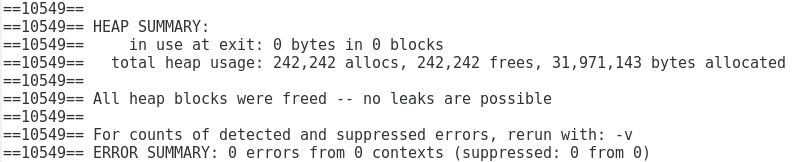
\includegraphics[width=0.8\textwidth]{figuras/monitorWebCliTeste1/resultado5.JPG}
	\caption[Resultado do Valgrind com configuração comum.]{Resultado do Valgrind com configuração comum. Pode ser visto que todas as memórias que foram alocadas pela aplicação foram desalocadas e que zero erros foram encontrados em zero contextos diferentes.}
	\label{Img:resultado5Valgrind}
\end{figure}



Na \autoref{Img:ConsumoDoSistema} pode ser visto o consumo de recursos do \textit{hardware} que a aplicação MonitoreWeb-Cli estava consumindo durante os 5 minutos de execução de um dos testes. Nela pode ser observado o uso do processador (\%CPU) que foi crescendo gradualmente até se estabilizar em 0,5\% tendo uma media de 0,44\% e desvio padrão de 0.09057\%. O mesmo pode ser observado com a memória virtual (VSZ), que foi estabilizada em 906960 (0.864944 Mb). Outro valor a ser observado é o tempo total da CPU utilizada pelo processo desde que foi iniciado (TIME), que ficou em aproximadamente 1 segundo dentro de um período de monitoramento de 5 minutos. A lista a seguir descreve o significado das principais colunas da figura.


%SERIA IDEAL APRESENTAR O CONSUMO MÉDIO. Média (Average)  Média (Average) 0.44,  Desvio padrão 0.09057
% 0.1,0.2,0.2,0.2,0.3,0.3,0.4,0.4,0.4,0.4,0.4,0.4,0.4,0.4,0.5,0.4,0.4,0.4,0.5,0.4,0.4,0.4,0.4,0.4,0.5,0.4,0.4,0.5,0.4,0.5,0.5,0.5,0.5,0.5,0.5,0.5,0.5,0.5,0.5,0.5,0.5,0.5,0.5,0.5,0.5,0.5,0.5,0.5,0.5,0.5,0.5,0.5,0.5,0.5,0.5,0.5,0.5,0.5,0.5,0.5  Média (Average) 0.44,  Desvio padrão 0.09057

\begin{itemize}
    \item PID: número de identificação do processo.
    
    \item \%CPU: consumo de processamento do processo.
    
    \item \%MEM: consumo de memória do processo.
     
    \item VSZ: tamanho da memória virtual, que corresponde à memória do processo mais a memória de bibliotecas compartilhadas.
    
    \item RSS: soma total da memória física usada pelo processo.
    
    \item TIME: tempo total da CPU usado pelo processo desde que foi iniciado.
        
    \item COMMAND: Nome do comando do processo.

\end{itemize}
\begin{figure}[H]
	\centering
	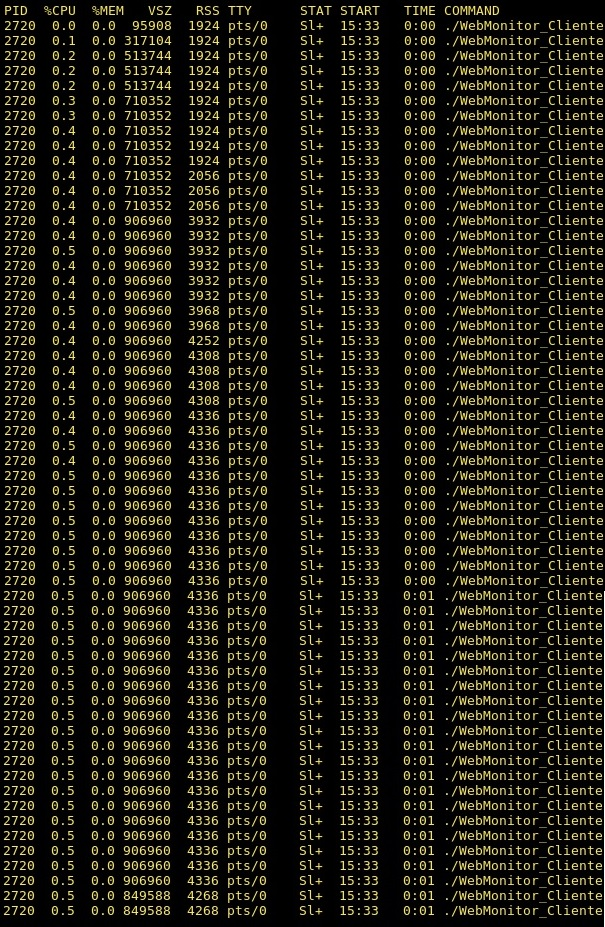
\includegraphics[width=0.8\textwidth]{figuras/monitorWebCliTeste1/hardware.JPG}
	\caption[Consumo de recursos do \textit{hardware} com a configuração comum.]{Consumo de recursos do \textit{hardware} com a configuração comum. A coluna \%CPU representa o consumo de processamento, esse valor foi estabilizado em 0,5\% tendo uma media de 0,44\% e desvio padrão de 0.09057\%.}
	\label{Img:ConsumoDoSistema}
\end{figure}



% # # # # # # # # # # # # # # # # # # # # # # # # # # # # # # # # # # # # # # # # # # # # # # # # # # # # # # # # # # # # # # # # # # # # # # # # # # # # # # # # # # # # # # # # # # # # # # # # # # # # # # # # # # # # # # # # # # # # # # # # # # # # # # # # # # # # # # # # # # # # # # # # # # # # # # # # # # # # # # # # # # # # # # # # # # # # # # # # # # # # # # # # # # # # # # # # # # # # # # # # # # # # # # # # # # # # 

\subsection{Testes com Configuração Extrema} \label{subsec:QuantidadeRequisicoesMaiores}

Esse teste teve como objetivo executar todas as operações do sistema cliente sem intervalos, causando uma situação extrema de processamento, uso de memória e uso do disco. Conforme descrito anteriormente, essa configuração não é recomendada devido ao fato de sobrecarregar a máquina cliente, sem apresentar contraponto relevante, uma vez que o monitoramento a cada 1s é suficiente para um monitoramento preciso. Essa configuração foi utilizada no teste com a intenção de gerar um processamento elevado, aumentando a possibilidade do Valgrid detectar falhas. O teste foi repetido 5 vezes, tendo um tempo de duração de 5 minutos. As configurações principais do sistema cliente encontra-se na \autoref{Tab:ConfiguraçãoExtrema}.


\begin{table}[H]
\centering
\label{my-label}
\begin{tabular}{|l|c|}
\hline
\multicolumn{1}{|c|}{{\color[HTML]{000000} \textbf{Configuração}}} & {\color[HTML]{000000} \textbf{Intervalo}} \\ \hline
Envio do registro de monitoramento da CPU                 & 0s                                                                        \\ \hline
Envio do registro de monitoramento da memória             & 0s                                                                        \\ \hline
Envio do registro de monitoramento da \textit{swap}                & 0s                                                                        \\ \hline
Realização da leitura das configurações do servidor       & 1s                                                                       \\ \hline
Envio do registro de monitoramento do PostgreSQL          & 30s                                                                       \\ \hline
Envio do registro de um procedimento de \textit{vacuum}   & 30s                                                                       \\ \hline
Envio do registro de um procedimento de \textit{backup}   & 30s                                                                       \\ \hline
\end{tabular}
\caption[Principais valores da configuração extrema.]{Principais valores da configuração extrema.}
\label{Tab:ConfiguraçãoExtrema}
\end{table}

O resultado foi satisfatório, nenhuma das 5 execuções do teste apresentaram defeito. O relatório apresentado pela ferramenta Valgrind pode ser visto na \autoref{Img:resultado5Valgrindteste2}.

\begin{figure}[H]
	\centering
	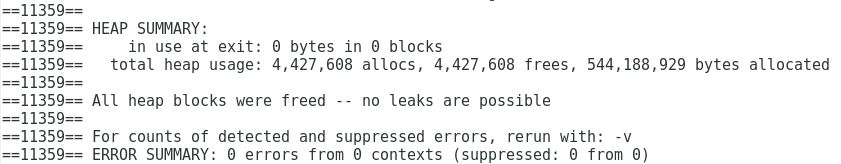
\includegraphics[width=1.0\textwidth]{figuras/monitorWebCliTeste2/resultado5 minutos.jpg}
	\caption[Resultado do Valgrind com processamento extremo.]{Resultado do Valgrind com processamento extremo. Cabe observar que toda a memória alocada pela aplicação foi desalocada, e que zero erros foram encontrados.}
	\label{Img:resultado5Valgrindteste2}
\end{figure}

%SERIA IDEAL APRESENTAR O CONSUMO MÉDIO. Média (Average) 25.99016, Desvio padrão 4.4445
% 3.2,11.1,14.4,16.1,19.3,21.8,22.4,23.1,24.9,25.7,26.4,26.5,26.7,26.7,26.9,27.2,27.3,27.3,27.5,27.5,27.5,27.5,27.5,27.5,27.5,27.5,27.5,27.5,27.5,27.4,27.4,27.2,27.2,27.2,27.3,27.3,27.3,27.4,27.4,27.5,27.5,27.6,27.6,27.7,27.7,27.7,27.7,27.8,27.8,27.9,27.9,27.9,27.9,28,28,28,28,28.1,28.1,28.2,28.2   https://www.easycalculation.com/pt/statistics/standard-deviation.php  Média (Average) 25.99016, Desvio padrão 4.4445

Na \autoref{Img:consumo2} mostra-se o consumo de recursos do \textit{hardware} que a aplicação MonitoreWeb-Cli consumiu durante os 5 minutos da execução de um dos testes. Nela, o uso do processador (\%CPU) foi crescendo gradualmente até se estabilizar em aproximadamente 27,5\% tendo uma média de 25.99016\% e desvio padrão de 4.4445\%. O mesmo pode ser observado com a memória virtual (VSZ), que foi estabilizada em 906960 (0.864944 Mb) - mesmo resultado do teste da \autoref{subsec:QuantidadeRequisicoesNormais}. Outro valor a ser observado é o tempo que o sistema dedicou exclusivamente para a aplicação (TIME), que ficou em aproximadamente 1 minuto e 26 segundos em um período total de monitoramento de 5 minutos.

\begin{figure}[H]
	\centering
	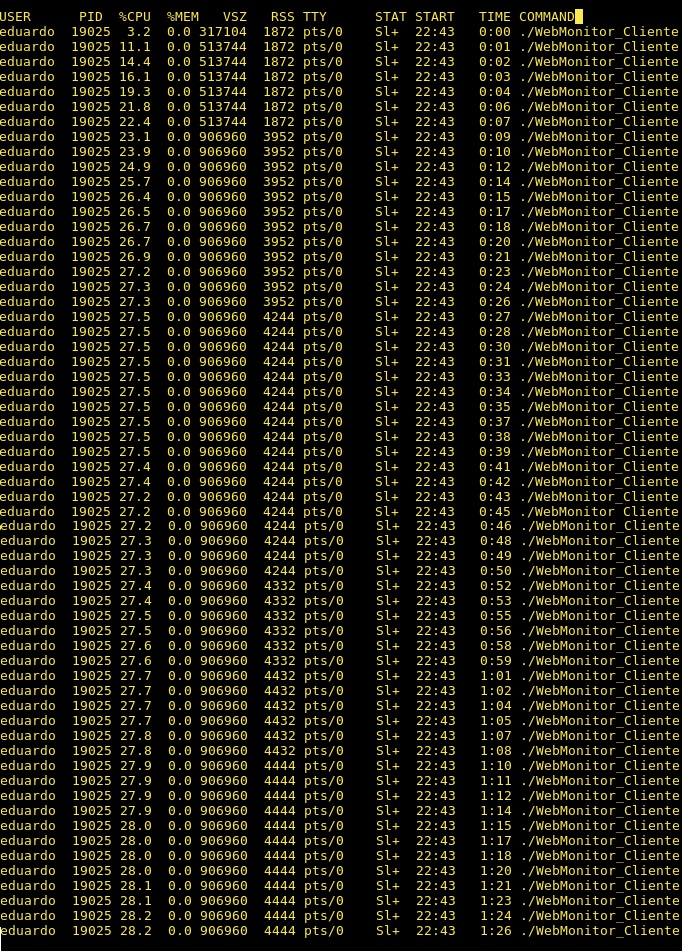
\includegraphics[width=0.8\textwidth]{figuras/monitorWebCliTeste2/hardwareTeste2.jpg}
	\caption[Consumo de recursos do \textit{hardware} com configuraçãos extremas.]{Consumo de recursos do \textit{hardware} com configurações extremas.  A coluna \%CPU representa o consumo de processamento, esse valor foi estabilizado em torno de 27,5\% tendo uma media de 25.99016\% e desvio padrão de 4.4445\%}
	\label{Img:consumo2}
\end{figure}


\section{MonitorWeb-Api} \label{sec:MonitorWeb-ApiTeste}

Nesta seção descreve-se os testes unitários, vistos anteriormente na \autoref{sec:TestesAutomatizados}. Estes, tiveram o intuído de trazer a confiabilidade de que todos os recursos da aplicação funcionam corretamente. Além disso, foi realizado testes para verificar o desempenho (em termos de uso de memória e de CPU, e quantidade de requisições atendidas) do servidor web durante diferentes cargas de requisição.

\subsection{Testes de Unidade}\label{}

Para a realização dos teste de unidade foi utilizado a ferramenta Spring Boot Test, vista na \autoref{subsec:SpringTest}. Todos os teste citados nesta subseção podem ser encontrados no pacote \url{/src/test} do projeto.

Foram realizados testes de unidade para todos os recursos da aplicação. Os testes foram realizados de acordo com a funcionalidade de cada recurso. A \autoref{Img:PlanilhaTesteUnidade} mostra quais testes foram realizados em cada recurso da aplicação.

Os testes descritos na lista a seguir fazem os seguintes procedimentos:

\begin{itemize}
    \item buscarPorIdTest: efetua uma busca por id e verifica se o objeto recebido corresponde ao objeto desejado.
    
    \item buscarTodosTest: efetua uma busca e verifica se todos os objetos do banco de dados foram trazidos com sucesso.
    
    \item buscarTodosPorServidorTest: efetua uma busca por id de um Objeto Servidor e verifica se os valores obtidos são os desejados.
    
    \item buscarIdInexistenteServidorTest: efetua uma busco por id de um Objeto Servidor inexistente e verifica se retorna o valor esperado.
    
    \item deletarTest: deleta um registo e verifica se ele foi realente deletado.
    
    \item deletarIdInexistenteTest: tenta deletar um registro que não existe e verifica se o sistema retorna o valor esperado.
    
    \item inserirTest: insere um registro e verifica se os valores inseridos estão corretos.
\end{itemize}
 

\begin{figure}[H]
	\centering
	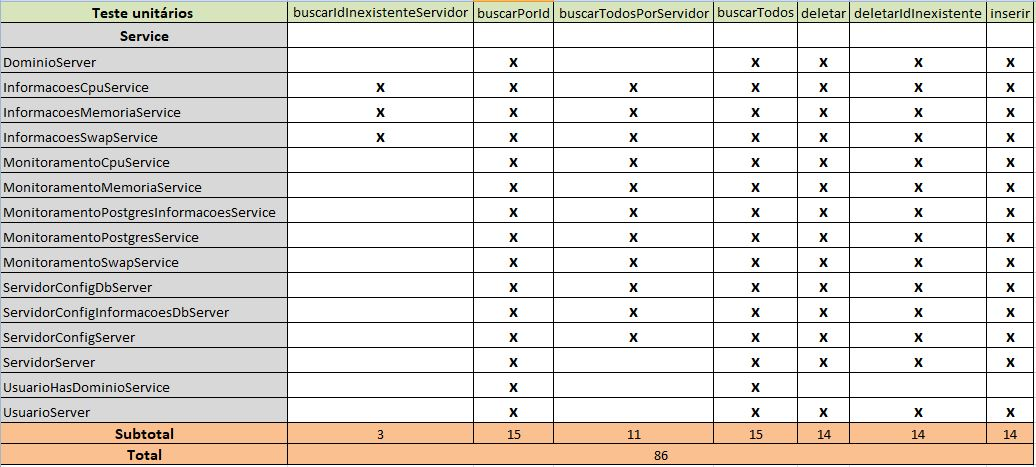
\includegraphics[width=1.0\textwidth]{figuras/MonitorWebApiTeste3/Teste3Planilha.jpg}
	\caption[Planilha de intersecção dos testes de unidade com services]{Planilha de intersecção dos testes de unidade com services, onde a intersecção representada pela letra X indica que o teste foi realizado.}
	\label{Img:PlanilhaTesteUnidade}
\end{figure}


Na \autoref{Img:testeUnitarioOk} pode ser visto todos os 86 testes unitários executados com sucesso.

\begin{figure}[H]
	\centering
	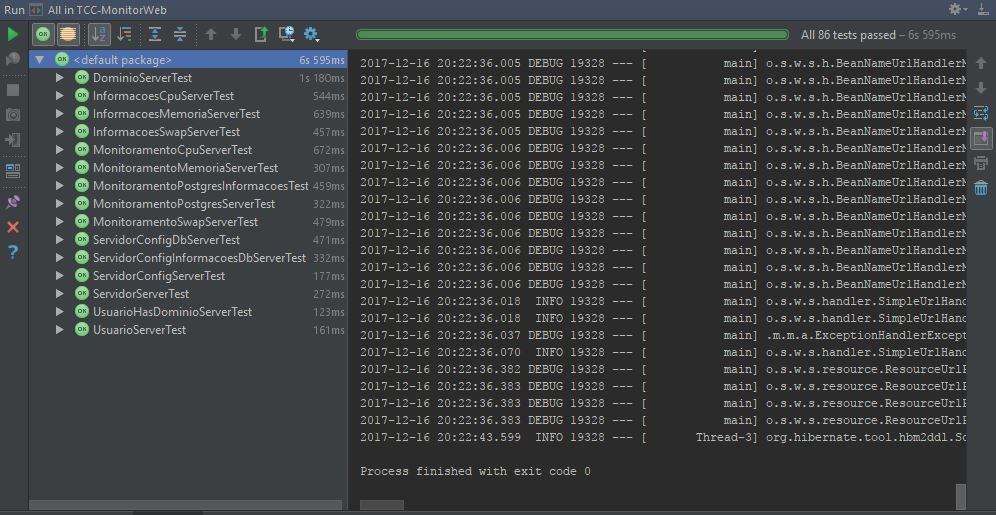
\includegraphics[width=1.0\textwidth]{figuras/MonitorWebApiTeste3/ResultadoTeste2.jpg}
	\caption[IntelliJ executando os 86 testes de unidade com sucesso]{IntelliJ executando os 86 testes de unidade com sucesso}
	\label{Img:testeUnitarioOk}
\end{figure}


\subsection{Teste de Desempenho do MonitorWeb-Api} \label{}

Os teste apresentados nesta seção tem como objetivo medir o desempenho da aplicação MonitorWeb-Api, verificando sua capacidade de monitoramento e consumo de recursos do \textit{hardware}.

Para execução desse teste, foi utilizado dois computadores: um executando a aplicação servidor (MonitorWeb-Api) e outro executando a aplicação cliente (MonitorWeb-Cli).

\begin{itemize}
    \item MonitorWeb-Api: computador com processador Intel i7-4500U (1.80GHz a 3.00GHz, Cache de 4MB), memória de 16GB (DDR3 1600MHz), SDD de 480GB (Modelo SA400S37480G, capacidade de leitura: 500MBs/s, capacidade de gravação: 450MB/s) e sistema operacional Windows 10 Professional.
    
    \item MonitorWeb-Cli: computador com processador Intel i5-7200U (2.50GHz a 3.1GHz, Cache de 3MB), memória de 8GB (DDR4 2400MHz) e sistema operacional Debian 9 Stretch (Linux Kernel 4.9).
\end{itemize}

\subsubsection{Quantidade de consumo com a configuração comum} \label{subsec:APIQuantidadeRequisicoesNormais}

Esse teste teve o objetivo de executar a aplicação MonitorWeb-Api juntamente com o sistema cliente. As configurações utilizadas para o sistema cliente foram as mesmas do teste com as configurações comum mostrado na \autoref{subsec:QuantidadeRequisicoesNormais}.

Na \autoref{Img:BaixoProcessametno} mostra-se dois gráficos: no primeiro apresenta-se o consumo de memória (\textit{memory}) e no segundo apresenta-se consumo de CPU (\textit{CPU Load}), tendo o teste a duração de 8 minutos. Do minuto 0:00 ao 0:16 a aplicação estava sendo iniciada; do 0:16 ao 1:06 ficou em estado de espera por uma aplicação cliente; no minuto 1:07, foi iniciada a comunicação com a aplicação cliente que durou até o minuto 7:00. Após isso, a aplicação cliente terminou.

\begin{figure}[H]
	\centering
	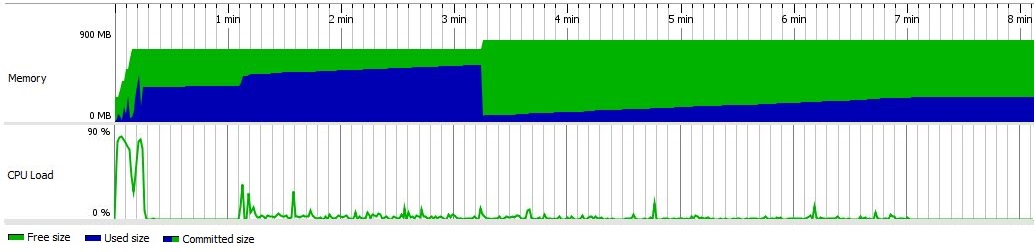
\includegraphics[width=1.0\textwidth]{figuras/MonitorWebApiTeste4/BaixoProcessametno.jpg}
	\caption[Quantidade de consumo com a configuração comum]{Quantidade de consumo do sistema MonitorWeb-Api com a configuração comum. Dois gráficos podem ser vistos na figura. O primeiro representa o consumo de memoria da aplicação servidor e o segundo o consumo de CPU.}
	\label{Img:BaixoProcessametno}
\end{figure}



\subsubsection{Teste com Processamento Extremo}\label{subsec:APIQuantidadeRequisicoesMaior}


Neste teste, as configurações utilizadas para o sistema cliente foram as mesmas da \autoref{subsec:QuantidadeRequisicoesMaiores}, entretanto, não houve intervalo entre as consultas de monitoramento, e dessa forma, pode-se analisar o comportamento das duas aplicações sobre uma carga de processamento extrema.

Na figura \autoref{Img:BaixoProcessametno} apresenta-se dois gráficos: o primeiro sobre o consumo de memória (\textit{memory}) e o segundo sobre consumo de CPU (\textit{CPU Load}) com duração de 9 minutos. Do minuto 0:00 ao 0:16 a aplicação estava sendo iniciada; do 0:16 ao 1:12 a aplicação estava esperando por uma aplicação cliente para iniciar a comunicação; no minuto 1:13 é iniciado a comunicação com a aplicação cliente, que durou até o minuto 8:30. Após isso, a aplicação cliente foi encerrada.

\begin{figure}[H]
	\centering
	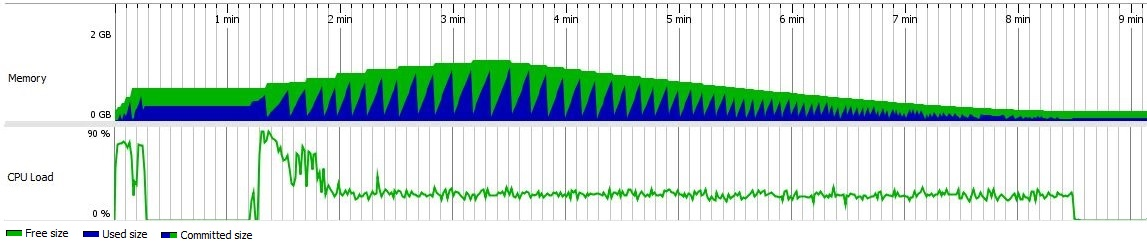
\includegraphics[width=1.0\textwidth]{figuras/MonitorWebApiTeste4/AutoProcessametno.jpg}
	\caption[Quantidade de consumo com a configuração extrema]{Quantidade de consumo do sistema MonitorWeb-Api com a configuração extrema. Dois gráficos podem ser vistos na figura. O primeiro representa o consumo de memoria da aplicação servidor e o segundo o consumo de CPU}
	\label{Img:AutoProcessametno.jpg}
\end{figure}

Na figura \autoref{Img:GerenciadorDoWindows5} e na \autoref{Img:GerenciadorDoWindows5-2.jpg} pode ser observado que o banco de dados PostgreSQL teve grande contribuição para o SSD atingir 100\% de seu desempenho, gerando um gargalo para a aplicação. 

Na figura \autoref{Img:sql1.jpg} mostra-se a quantidade de registros inseridos no banco de dados no intervalo de 7:17 minutos. Neste período, foram inseridos no banco de dados 76911 registros de CPU, 80078 registros de memória e 81762 registros \textit{swap}, o que dá, respectivamente, uma taxa de 175,99/s, 183,24/s, e 187,09/s. Esses valores totalizam em média, a inserção de 546,34 registros por segundos.

\begin{figure}[H]
	\centering
	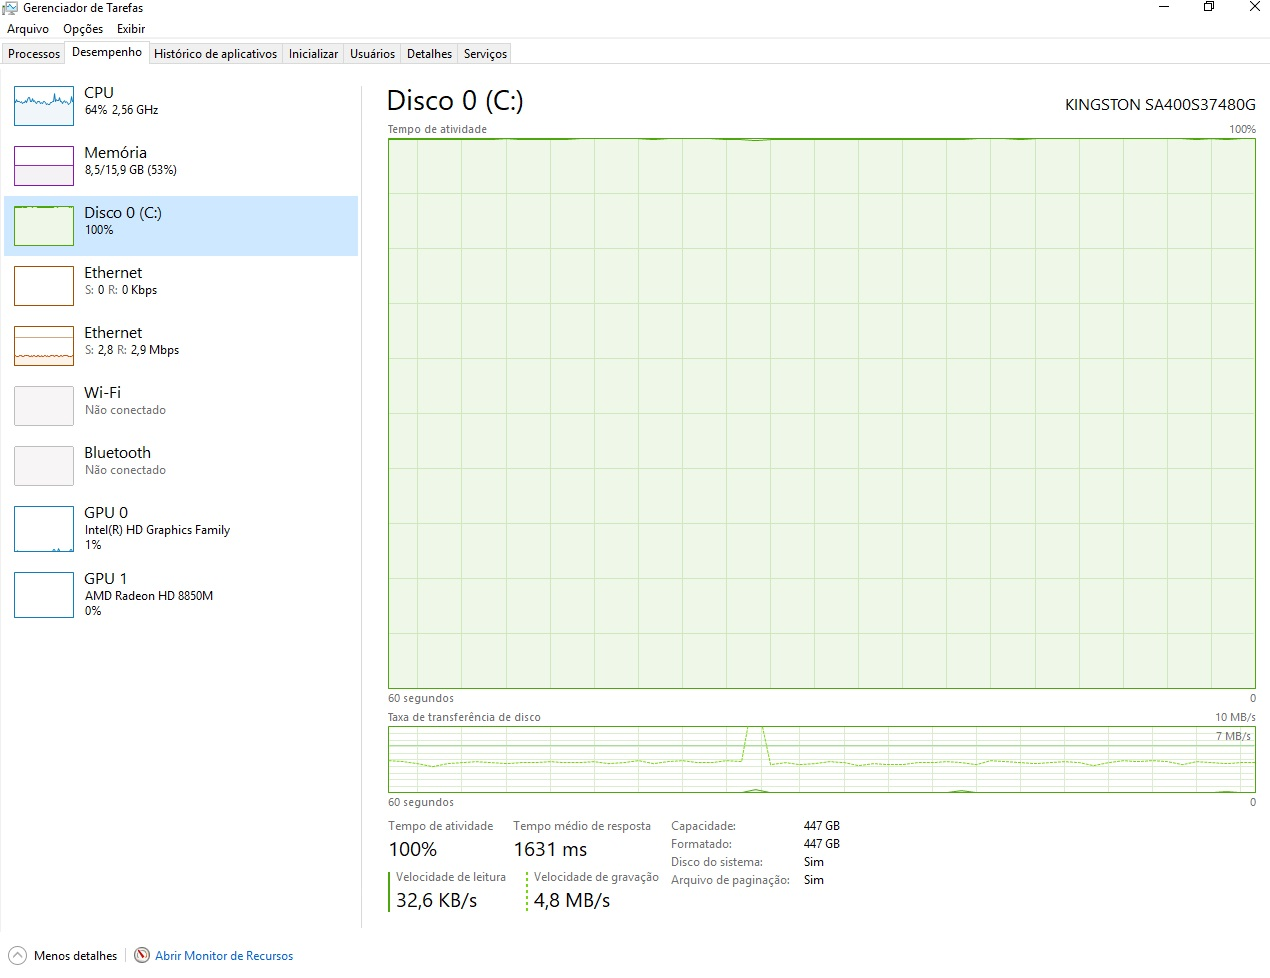
\includegraphics[width=1.0\textwidth]{figuras/MonitorWebApiTeste4/GerenciadorDoWindows5.jpg}
	\caption[Gerenciador de tarefas do Windows mostrando o consumo de recursos]{Gerenciador de tarefas do Windows mostrando o consumo do SSD em 100\%}
	\label{Img:GerenciadorDoWindows5}
\end{figure}

\begin{figure}[H]
	\centering
	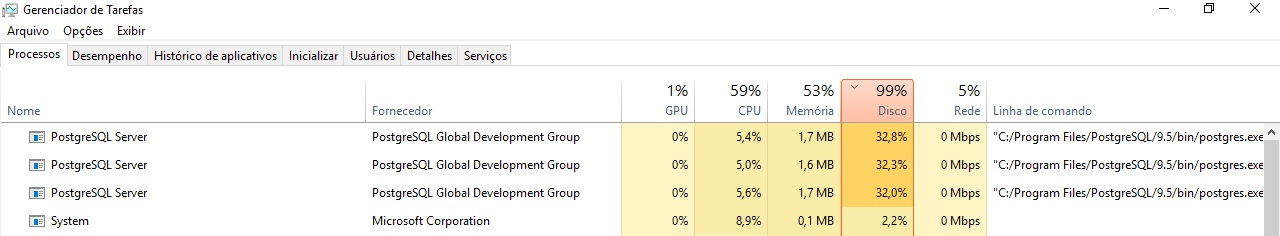
\includegraphics[width=1.0\textwidth]{figuras/MonitorWebApiTeste4/GerenciadorDoWindows5-2.jpg}
	\caption[Gerenciador de tarefas do Windows mostrando os principais processos]{Gerenciador de tarefas do Windows mostrando os principais processos}
	\label{Img:GerenciadorDoWindows5-2.jpg}
\end{figure}

\begin{figure}[H]
	\centering
	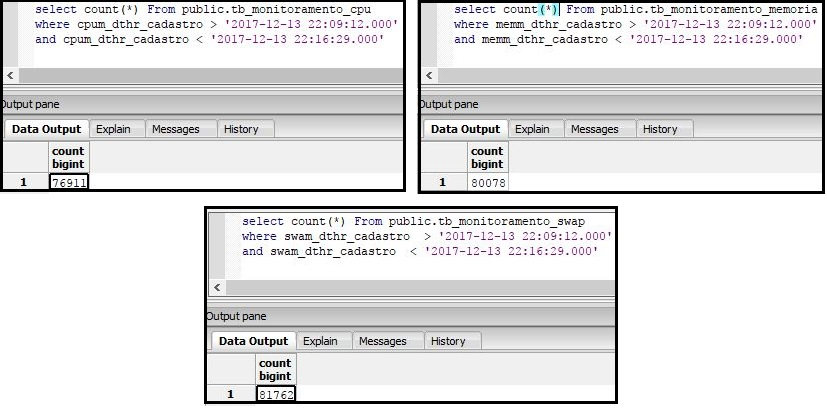
\includegraphics[width=1.0\textwidth]{figuras/MonitorWebApiTeste4/sql1.jpg}
	\caption[Quantidade de registros inseridos no banco de dados.]{Quantidade de registros inseridos no banco de dados no intervalo de 7:17 minutos.}
	\label{Img:sql1.jpg}
\end{figure}
 % Resultados
%====================================================================================================
% Monitoramento de servidores Linux por web sites.
%====================================================================================================
% Plano de Trabalho
%----------------------------------------------------------------------------------------------------
% Autor					: Eduardo Balan
% Orientador		: Kleber Kruger
% Instituição 	: UFMS - Universidade Federal do Mato Grosso do Sul
% Unidade				: CPCX - Campus de Coxim
%----------------------------------------------------------------------------------------------------
% Arquivo			: plano_trabalho.tex
% Data de criação	: 29 de Março de 2017
%=====================================================================================================

\chapter{Conclusão} \label{cap:conclusao}

 % Conclusão

\cleardoublepage
\phantomsection
\addcontentsline{toc}{chapter}{Referências Bibliográficas}
\bibliographystyle{abnt}
%\bibliographystyle{apalike} 
%\bibliographystyle{ieeetr} % Ordena por ordem de aparição.  
%\bibliographystyle{abbr} % Ordena por ordem alfabetica com nomes abreviados.
%\bibliographystyle{plain} % Ordena por ordem alfabetica com nomes por extenso.
\bibliography{bibliografia} % commented if *.bbl file included.

\addcontentsline{toc}{chapter}{Ap\^endices}
\appendix
% Monitoramento de servidores Linux por web sites.
%====================================================================================================
% TCC
%----------------------------------------------------------------------------------------------------
% Autor				    : Eduardo Balan
% Orientador		  : Kleber Krugrer
% Instituição 		: UFMS - Universidade Federal do Mato Grosso do Sul
% Departamento		: CPCX - Sistema de Informação
%----------------------------------------------------------------------------------------------------
% Data de criação	: 29 de Março de 2017
%====================================================================================================

\chapter{Anexos} \label{App:ApendiceA}


\begin{table}[!ht]
\centering
\begin{tabular}{|l|l|}
\hline
{\color[HTML]{000000} \textbf{Variável}} & {\color[HTML]{000000} \textbf{Descrição}}                                      \\ \hline
id                                       & Número único para cada objeto do tipo ServidorConfig.\\ 
																				 &(Gerado Automaticamente) 																												\\ \hline
servidor                                 & Indica com qual objeto Servidor esse registro esta relacionado.                       \\ \hline
dthr\_cadastro                           & Data e hora do cadastro. (Gerado Automaticamente)                              \\ \hline
nome                                     & Nome do processador.                                                           \\ \hline
cacheSize                                & Tamanho do cache do processador.                                               \\ \hline
cpuCores                                 & Quantos núcleos tem o processador.                                             \\ \hline
siblings                                 & Quantos núcleos virtuais tem o processador.                                    \\ \hline
\end{tabular}
\caption[Variáveis da classe InformacoesCpu e suas descrições.]{Variáveis da classe InformacoesCpu e suas descrições.}
\label{Tab:VariaveisInformacoesCpu}
\end{table}



\begin{table}[!ht]
\centering
\begin{tabular}{|l|l|}
\hline
{\color[HTML]{000000} \textbf{Variável}} & {\color[HTML]{000000} \textbf{Descrição}}                                      \\ \hline
id                                       & Número único para cada objeto do tipo ServidorConfig.\\ 
																				 &(Gerado Automaticamente) 																												\\ \hline
servidor                                 & Indica com qual objeto Servidor esse registro esta relacionado.                       \\ \hline
dthr\_cadastro                           & Data e hora do cadastro. (Gerado Automaticamente)                              \\ \hline
total                                    & Quanto de memoria existe no servidor.                                          \\ \hline
\end{tabular}
\caption[Variáveis da classe InformacoesMemoria e suas descrições.]{Variáveis da classe InformacoesMemoria e suas descrições.}
\label{Tab:VariaveisInformacoesMemoria}
\end{table}


\begin{table}[!ht]
\centering
\begin{tabular}{|l|l|}
\hline
{\color[HTML]{000000} \textbf{Variável}} & {\color[HTML]{000000} \textbf{Descrição}}                                      \\ \hline
id                                       & Número único para cada objeto do tipo ServidorConfig.\\ 
																				 &(Gerado Automaticamente) 																												\\ \hline
servidor                                 & Indica com qual objeto Servidor esse registro esta relacionado.                       \\ \hline
dthr\_cadastro                           & Data e hora do cadastro. (Gerado Automaticamente)                              \\ \hline
total                                    & Quanto de memoria swap existe no servidor.                                     \\ \hline
\end{tabular}
\caption[Variáveis da classe InformacoesSwap e suas descrições.]{Variáveis da classe InformacoesSwap e suas descrições.}
\label{Tab:VariaveisInformacoesSwap}
\end{table}


\begin{table}[!ht]
\centering
\begin{tabular}{|l|l|}
\hline
{\color[HTML]{000000} \textbf{Variável}} & {\color[HTML]{000000} \textbf{Descrição}}                                      \\ \hline
id                                       & Número único para cada objeto do tipo ServidorConfig.\\ 
																				 &(Gerado Automaticamente) 																												\\ \hline
informacoesCpu                           & Indica com qual objeto InformacoesCpu esse registro \\ 
																				 &esta relacionado.          \\ \hline
dthr\_cadastro                           & Data e hora do cadastro. (Gerado Automaticamente)                              \\ \hline
coreId                                   & Id do núcleo que esta sendo monitorado.                                        \\ \hline
cpuMhz                                   & Quantos Mhz (MegaHertz) esta sendo utilizado.                                  \\ \hline
\end{tabular}
\caption[Variáveis da classe MonitoramentoCpu e suas descrições.]{Variáveis da classe MonitoramentoCpu e suas descrições.}
\label{Tab:VariaveisMonitoramentoCpu}
\end{table}

\begin{table}[!ht]
\centering
\begin{tabular}{|l|l|}
\hline
{\color[HTML]{000000} \textbf{Variável}} & {\color[HTML]{000000} \textbf{Descrição}}                                                                             \\ \hline
id                                       & \multicolumn{1}{p{10.00cm}|}{Número único para cada objeto do tipo ServidorConfig. (Gerado Automaticamente)}                                        \\ \hline
informacoesMemoria                       & \multicolumn{1}{p{10.00cm}|}{Indica com qual objeto InformacoesMemoria esse registro esta relacionado. }\\ \hline
dthr\_cadastro                           & \multicolumn{1}{p{10.00cm}|}{Data e hora do cadastro. (Gerado Automaticamente)} \\ \hline
active                                   & \multicolumn{1}{p{10.00cm}|}{A quantidade total de buffer (Memoria Temporaria) ou memória cache que foi utilizada recentemente e não foi liberada.} \\ \hline
memfree                                  & \multicolumn{1}{p{10.00cm}|}{A quantidade de  memoria física não utilizada.} \\ \hline
availabre                                & \multicolumn{1}{p{10.00cm}|}{A quantidade de memoria que pode ser acessada pelo servidor.} \\ \hline
buffers                                  & \multicolumn{1}{p{10.00cm}|}{A quantidade de memoria física utilizada para buffers  de arquivos.}   \\ \hline
\end{tabular}
\caption[Variáveis da classe MonitoramentoMemoria e suas descrições.]{Variáveis da classe MonitoramentoMemoria e suas descrições.}
\label{Tab:VariaveisMonitoramentoMemoria}
\end{table}

\begin{table}[!ht]
\centering
\begin{tabular}{|l|l|}
\hline
{\color[HTML]{000000} \textbf{Variável}} & {\color[HTML]{000000} \textbf{Descrição}}                                      \\ \hline
id                                       & \multicolumn{1}{p{10.00cm}|}{Número único para cada objeto do tipo ServidorConfig. (Gerado Automaticamente)}\\ \hline
InformacoesSwap                          & Indica com qual objeto InformacoesSwap esse registro esta  \\
																				 & relacionado.         \\ \hline
dthr\_cadastro                           & Data e hora do cadastro. (Gerado Automaticamente)                              \\ \hline
free                                     & O montante total de swap livre.                                                \\ \hline
cached                                   & A quantidade de swap que esta sendo utilizada.                                 \\ \hline
\end{tabular}
\caption[Variáveis da classe MonitoramentoSwap e suas descrições.]{Variáveis da classe MonitoramentoSwap e suas descrições.}
\label{Tab:VariaveisMonitoramentoSwap}
\end{table}


\begin{table}[!ht]
\centering
\begin{tabular}{|l|l|}
\hline
{\color[HTML]{000000} \textbf{Variável}} & {\color[HTML]{000000} \textbf{Descrição}}\\ \hline
id                                       &  \multicolumn{1}{p{10.00cm}|}{Número único para cada objeto do tipo ServidorConfigDb. (Gerado Automaticamente)} \\ \hline
servidorConfigDb                         &  \multicolumn{1}{p{10.00cm}|}{Indica com qual objeto ServidorConfigDb esse registro esta relacionado.} \\ \hline
dthr\_cadastro                           &  \multicolumn{1}{p{10.00cm}|}{Data e hora do cadastro. (Gerado Automaticamente)} \\ \hline
tipoExecucao                             &  \multicolumn{1}{p{10.00cm}|}{É uma enum do tipo EnumSgdbTipoExec o qual informa se o procedimento é um backup ou um vacuum. }\\ \hline
exito                                    &  \multicolumn{1}{p{10.00cm}|}{Informa se a procedimento foi realizado com sucesso. }\\ \hline
mensagem                                 &  \multicolumn{1}{p{10.00cm}|}{Mensagem gerada pelo procedimento. }\\ \hline
\end{tabular}
\caption[Variáveis da classe MonitoramentoPostgres e suas descrições.]{Variáveis da classe MonitoramentoPostgres e suas descrições.}
\label{Tab:VariaveisMonitoramentoPostgres}
\end{table}

\begin{table}[!ht]
\centering
\begin{tabular}{|l|l|}
\hline
{\color[HTML]{000000} \textbf{Variável}} & {\color[HTML]{000000} \textbf{Descrição}} \\ \hline
id                                       & \multicolumn{1}{p{10.00cm}|}{Número único para cada objeto do tipo ServidorConfigDb. (Gerado Automaticamente)}\\ \hline
ServidorConfigInformacoesDb              & \multicolumn{1}{p{10.00cm}|}{Indica com qual objeto ServidorConfigInformacoesDb esse registro esta relacionado. }\\ \hline
dthr\_cadastro                           & \multicolumn{1}{p{10.00cm}|}{Data e hora do cadastro. (Gerado Automaticamente)  }\\ \hline
listenAddresses                          & \multicolumn{1}{p{10.00cm}|}{De qual ip o postgreSQL ira aceitar conexão.}\\ \hline
port                                     & \multicolumn{1}{p{10.00cm}|}{Porta que o postgreSQL esta rodando.}\\ \hline
maxConnections                           & \multicolumn{1}{p{10.00cm}|}{Numero máximo de conexão que o postgresSQL ira aceitar simultaneamente. }\\ \hline
ssl                                      & \multicolumn{1}{p{10.00cm}|}{Se a conexão com o banco possui ssl (Secure Socket Layer). }\\ \hline
sharedBuffers                            & \multicolumn{1}{p{10.00cm}|}{Quantidade de memória compartilhada utilizada pelo postgreSQL.}\\ \hline
tempBuffers                              & \multicolumn{1}{p{10.00cm}|}{Quantidade de memória utilizada por sessão do postgresSQL.}\\ \hline
workMem                                  & \multicolumn{1}{p{10.00cm}|}{Quantidade de memória utilizada por operações de classificação interna e tabelas de hash antes de gravar em arquivos de disco.  }\\ \hline
maintenanceWorkMem                       & \multicolumn{1}{p{10.00cm}|}{Quantidade máxima de memória a ser usada por operações de manutenção, como VACUUM , CREATE INDEX e ALTER TABLE ADD FOREIGN KEY. }\\ \hline
maxStackDepth                            & \multicolumn{1}{p{10.00cm}|}{Especifica a profundidade máxima da pilha de execução do postgresSQL no servidor.}\\ \hline
maxPreparedTransactions                  & \multicolumn{1}{p{10.00cm}|}{Define o número máximo de transações que podem estar no estado "prepared".} \\ \hline
\end{tabular}
\caption[Variáveis da classe ServidorConfigInformacoesDb e suas descrições.]{Variáveis da classe ServidorConfigInformacoesDb e suas descrições.}
\label{Tab:VariaveisMonitoramentoPostgres}
\end{table}


\begin{table}
\centering
\begin{tabular}{|l|l|}
\hline
{\color[HTML]{000000} \textbf{Variável}} & {\color[HTML]{000000} \textbf{Descrição}}                                        \\ \hline
id                                       & Número único para cada objeto do tipo ServidorConfigDb. \\
																				 & (Gerado Automaticamente) 																												\\ \hline
dthr\_cadastro                           & Data e hora do cadastro. (Gerado Automaticamente)                                \\ \hline
nome                                     & Nome do usuário.                                                                 \\ \hline
sobrenome                                & Sobrenome do usuário.                                                            \\ \hline
login                                    & Login do usuário.                                                                \\ \hline
email                                    & Email do usuário.                                                                \\ \hline
senha                                    & Senha de acesso do usuário.                                                      \\ \hline
sexo                                     & Enum do tipo EnumSexo para informar o sexo do usuário.                           \\ \hline
telefone                                 & Telefone para contato com o usuário.                                             \\ \hline
\end{tabular}
\caption[Variáveis da classe Usuario e suas descrições.]{Variáveis da classe Usuario e suas descrições.}
\label{Tab:VariaveisUsuario}
\end{table}


\begin{table}[!ht]
\centering
\begin{tabular}{|l|l|}
\hline
{\color[HTML]{000000} \textbf{Variável}} & {\color[HTML]{000000} \textbf{Descrição}}                                        \\ \hline
id                                       & Número único para cada objeto do tipo ServidorConfigDb.\\
																				 & (Gerado Automaticamente) \\ \hline
dthr\_cadastro                           & Data e hora do cadastro. (Gerado Automaticamente)                                \\ \hline
nome                                     & Nome do Dominio.                                                                 \\ \hline
observacao                               & Observação para o dominio.                                                       \\ \hline
\end{tabular}
\caption[Variáveis da classe Dominio e suas descrições.]{Variáveis da classe Dominio e suas descrições.}
\label{Tab:VariaveisDominio}
\end{table}


\chapter{Anexos} \label{App:ApendiceB}

\begin{lstlisting}[style=Java, label=Func:GenericEntity,caption={[Entidade genérica da aplicação GenericEntity.]Entidade genérica da aplicação GenericEntity e suas funcionalidades.}]
package br.com.webmonitor.entity.Generic;

import java.io.Serializable;
import java.util.Date;
import java.util.Objects;

/**
 * Classe base para qualquer objeto serializável.
 *
 * @author Eduardo Balan
 *
 * @param <T> o tipo do atributo id
 */
public abstract class GenericEntity<T extends Serializable> implements Serializable {

    private static final long serialVersionUID = 1L;

    public abstract T getId();

    public abstract void setId(T id);

    public abstract Date getDthr_cadastro();

    public abstract void setDthr_cadastro(Date date);

    /**
     * Indica quando outro objeto é igual a este. Nesta implementação, qualquer objeto derivado de Bean é igual a este desde que seja exatamente da mesma classe e tenha o mesmo ID.
     *
     * @author Kleber Kruger
     *
     * @param obj o objeto a comparar com este
     * @return {@code true} se este objeto é igual ao do argumento; {@code false} caso contrário.
     */
    @Override
    public boolean equals(Object obj) {
        if (getId() != null && obj instanceof GenericEntity) {
            GenericEntity x = (GenericEntity) obj;
            return getClass() == x.getClass() && getId().equals(x.getId());
        }
        return super.equals(obj);
    }

    /**
     * Retorna um valor de hash code para este objeto. Nesta implementação, este valor é gerado por
     * uma combinação do hash code da classe (getClass().hashCode()) somado ao hash code do atributo
     * id (id.hashCode()).
     *
     * @author Kleber Kruger
     *
     * @return um valor de hash code para este objeto
     */
    @Override
    public int hashCode() {
        if (getId() != null) {
            return 43 * 7 + Objects.hashCode(getClass().hashCode() + getId().hashCode());
        }
        return super.hashCode();
    }

}
\end{lstlisting}

\begin{lstlisting}[style=Java, label=Func:GenericBO,caption={[Entidade genérica GenericBO.]Entidade genérica GenericBO e suas funcionalidades.}]
package br.com.webmonitor.business.generic;

import br.com.webmonitor.entity.Generic.GenericEntity;
import br.com.webmonitor.exception.SqlGenericRuntimeException;
import br.com.webmonitor.exception.SqlInexistenteRuntimeException;
import org.springframework.beans.factory.annotation.Autowired;
import org.springframework.data.jpa.repository.JpaRepository;


import javax.persistence.MappedSuperclass;
import java.util.Date;


/**
 * Class GenericBO é a classe responsável  por regras de negocio, genéricos e simples como:
 * Inserção em uma base de dados, remoção da base de dados, e update.
 *
 * @author Eduardo Balan
 *
 * @param Entity Entidade a qual ela ira prestar o servico.
 * @param Repository Repositorio responsavel pela Entity que vc esta utilizando.
 *
 * @throws SqlInexistenteRuntimeException
 * @throws SqlGenericRuntimeException
 */
@MappedSuperclass
public class GenericBO <Entity extends GenericEntity, Repository extends JpaRepository<Entity, Long>> {

    /* Repositorio responsavel pela Entity */
    @Autowired
    private Repository repository;

    /**
     * Metodo responsável pelas regras de negocio genéricas da inserção.
     *
     * @author Eduardo Balan
     *
     * @param Entity Entidade que sera persistida no banco de dados.
     *
     * @throws SqlGenericRuntimeException
     *
     * return Entity persistida no banco de dados.
     */
    public Entity inserir(Entity entityNova){
        try{
            entityNova.setDthr_cadastro(new Date());
            return repository.save(entityNova);
        }catch (Exception e){
            throw new SqlGenericRuntimeException(e);
        }
    }

    /**
     * Metodo responsável pelas regras de negocio genéricas da exclusão.
     *
     * @author Eduardo Balan
     *
     * @param Long id da entidade que sera removida do banco de dados.
     *
     * @throws SqlInexistenteRuntimeException
     * @throws SqlGenericRuntimeException
     *
     * return void.
     */
    public void excluir(Long idEntity){
        Entity entityPersistidaNoDB = repository.findOne(idEntity);
        if(entityPersistidaNoDB == null){
            throw new SqlInexistenteRuntimeException("Registro não encontrado na base de dados.", null);
        }
        try{
            repository.delete(idEntity);
        }catch (Exception e){
            throw new SqlGenericRuntimeException(e);
        }
    }

}

}
\end{lstlisting}
%As tabelas deste apêndice mostram os resultados individuais dos testes sem a biblioteca \textit{FaultRecovery}, com a biblioteca \textit{FaultRecovery}, sem a classe \textit{TData} e com a classe \textit{TData}.

%\includepdf[pages={1-17}]{anexos.pdf}


%\documentclass[a4paper]{article}


\end{document}
